%IEEE template
\ifdefined\TTSTYLETARGETllncs
\documentclass{sty/llncs2e/llncs}
  %using latex.XXX file to cusotmize style
%customized tools
\usepackage{amssymb}
\usepackage{times}
\usepackage{amsfonts}
%\usepackage{amsthm}

\usepackage{subfig}
\usepackage{wrapfig}
\usepackage{float}
\usepackage{multirow, graphicx}
\usepackage{algorithm}
\usepackage{algpseudocode} %algorithm: use algorithmicx package, to refer to http://en.wikibooks.org/wiki/LaTeX/Algorithms_and_Pseudocode#Typesetting_using_the_algorithmicx_package
\usepackage{amsmath}

%squeeze space 
\setlength{\belowcaptionskip}{2pt}
\setlength{\abovecaptionskip}{2pt}
\setlength{\floatsep}{0.25\floatsep}
\setlength{\dblfloatsep}{0.25\dblfloatsep}
\setlength{\textfloatsep}{0.25 \textfloatsep}
\setlength{\dbltextfloatsep}{0.25\dbltextfloatsep}
\setlength{\intextsep}{0.25\intextsep}

%reduce whitespace surrounding section titles.
%\newcommand{\subparagraph}{} %from stackexchange: The titlesec package assumes all of the section levels provided by the standard classes are present. This includes the subparagraph level. The IEEEtrans class doesn't define a level subparagraph
%\usepackage[compact]{titlesec}  
%\titleformat{\paragraph}[runin]{\normalfont\itshape}{\theparagraph}{3pt}{} %keep paragraph title in the same line.
%TODO: to add manually a ":" to each of paragraph headings!

%TODO: to manually add \vspace{-.5cm} into authors and paper title, which reduce the whitespace in the front page.

%\usepackage{sty/simplemargins}
%    \setleftmargin{0.6in}
%    \setrightmargin{0.70in}
%    \settopmargin{0.55in}
%    \setbottommargin{0.55in}

%use to set line spacing for whole document
%f:http://en.wikibooks.org/wiki/LaTeX/Paragraph_Formatting#Line_spacing
%\usepackage{setspace} %dont use this alone (with sig-alternate)! footnote with 9 will show.
%\singlespacing
%\onehalfspacing
%\doublespacing
%\setstretch{1.1}


\usepackage{xspace}

%url
\usepackage{url}
\def\UrlBreaks{\do\/\do-}
\usepackage[breaklinks]{hyperref}
\usepackage{breakurl}

\usepackage{sty/widetext} %show equation in two columns

\usepackage{stackrel}

\let\oldemptyset\emptyset
\let\emptyset\varnothing

%cut words in middle when running out of space in a line.

%\pagestyle{empty} %this removes the page number
%\pagenumbering{gobble} %this really remove page numbers
\thispagestyle{plain}
\pagestyle{plain} %this enforce page number

\ifdefined\TTSTYLETARGETreport
% bibliography
\usepackage[
    backend=bibtex,
    maxbibnames=100,
    firstinits=true,
    bibstyle=numeric,
    citestyle=numeric
%    bibstyle=alphabetic,
%    citestyle=alphabetic
]{biblatex}
\addbibresource{ads.bib}
\addbibresource{lsm.bib}
\addbibresource{bkc.bib}
\addbibresource{dos.bib}
\addbibresource{odb.bib}
\addbibresource{cacheattacks.bib}
\addbibresource{sc.bib}
\addbibresource{crypto.bib}
\addbibresource{sgx.bib}
\addbibresource{diffpriv.bib}
\addbibresource{txtbk.bib}
\addbibresource{distrkvs.bib}
\addbibresource{vc.bib}
\addbibresource{yuzhetang.bib}
\fi

\usepackage{pifont}% http://ctan.org/pkg/pifont
\newcommand{\cmark}{\ding{51}}%
\newcommand{\xmark}{\ding{55}}%

%todonotes
\usepackage{todonotes}
\newcommand{\tangSide}[1]{\todo[caption={},color=cyan!20!]{{\tiny Note: #1}}}
\setlength{\marginparwidth}{1.5cm}
\newcommand{\ignore}[1]{}

\usepackage{graphicx, multirow}

%customized packages
\usepackage{tabularx, multirow, rotating} %tables, dependent on multirow package.
%rotating is used for \begin{sideways} environment
\usepackage{subfig} %figures
\usepackage{algorithm} %algorithm
\usepackage{algpseudocode} %algorithm: use algorithmicx package, to refer to http://en.wikibooks.org/wiki/LaTeX/Algorithms_and_Pseudocode#Typesetting_using_the_algorithmicx_package
%TOREMOVE \usepackage[noend]{algorithmic} %algorithm
\usepackage{ulem} % strike out text
\usepackage{color} % colored text

%for listing, like SQL
\usepackage{listings} 
\lstdefinestyle{Oracle}{basicstyle=\ttfamily,
                        keywordstyle=\lstuppercase,
                        emphstyle=\itshape,
                        showstringspaces=true,
                        }
\makeatletter
\newcommand{\lstuppercase}{\uppercase\expandafter{\expandafter\lst@token
                           \expandafter{\the\lst@token}}}
\newcommand{\lstlowercase}{\lowercase\expandafter{\expandafter\lst@token
                           \expandafter{\the\lst@token}}}
\makeatother


%for circled text
%f: http://tex.stackexchange.com/questions/7032/good-way-to-make-textcircled-numbers
\usepackage{tikz}
\newcommand*\circled[1]{\tikz[baseline=(char.base)]{
            \node[shape=circle,draw,inner sep=1pt] (char) {#1};}} 

%A white number inside a black circle.
% \usepackage{tikz}
\newcommand{\ballnumber}[1]{\tikz[baseline=(myanchor.base)] \node[circle,fill=.,inner sep=1pt] (myanchor) {\color{-.}\bfseries\footnotesize #1};}
%% use it
%\ballnumber{37}

%for boldening algorithm line numbers.
%f: http://tex.stackexchange.com/questions/99493/how-to-make-the-line-number-in-algorithm-shown-in-bold/99515#99515
\newif\ifboldnumber
\newcommand{\boldnext}{\global\boldnumbertrue}
% Default definition is \footnotesize#1:
\algrenewcommand\alglinenumber[1]{%
  \footnotesize\ifboldnumber\bfseries\fi\global\boldnumberfalse#1:}

%for rcases, or right brace
\newenvironment{rcases}
  {\left.\begin{aligned}}
  {\end{aligned}\right\rbrace}

%color table
\usepackage{color, colortbl}
%\definecolor{name}{system}{definition}
\definecolor{Gray}{gray}{0.9}
\definecolor{LightCyan}{rgb}{0.88,1,1}
\usepackage[first=0,last=9]{lcg}
\newcommand{\ra}{\rand0.\arabic{rand}}

%diagnal cross in table
%also require tikz package
\usepackage{colortbl}
\usetikzlibrary{calc}
\usepackage{zref-savepos}

\newcounter{NoTableEntry}
\renewcommand*{\theNoTableEntry}{NTE-\the\value{NoTableEntry}}

\newcommand*{\notableentry}{%
  \multicolumn{1}{@{}c@{}|}{%
    \stepcounter{NoTableEntry}%
    \vadjust pre{\zsavepos{\theNoTableEntry t}}% top
    \vadjust{\zsavepos{\theNoTableEntry b}}% bottom
    \zsavepos{\theNoTableEntry l}% left
    \hspace{0pt plus 1filll}%
    \zsavepos{\theNoTableEntry r}% right
    \tikz[overlay]{%
      \draw[red]
        let
          \n{llx}={\zposx{\theNoTableEntry l}sp-\zposx{\theNoTableEntry r}sp},
          \n{urx}={0},
          \n{lly}={\zposy{\theNoTableEntry b}sp-\zposy{\theNoTableEntry r}sp},
          \n{ury}={\zposy{\theNoTableEntry t}sp-\zposy{\theNoTableEntry r}sp}
        in
        (\n{llx}, \n{lly}) -- (\n{urx}, \n{ury})
        (\n{llx}, \n{ury}) -- (\n{urx}, \n{lly})
      ;
    }% 
  }%
}


\sloppy

  \begin{document}
% --- Author Metadata here ---
\title{
Title
\\ {\large \today}
\ifdefined\TTTOME
Tang's Paper Template \\ Title to be eye-catching for high citation: \\what's new \\short, \\mention approach (to researcher audience)
\fi
}


\author{
Kai Li\hspace{0.25cm}
Yuzhe (Richard) Tang\hspace{0.25cm}
Beom Heyn (Ben) Kim$\ ^\dag{}$\hspace{0.25cm}
Jianliang Xu$\ ^\ddag{}$\hspace{0.25cm}\\
\ifdefined\TTUT
\fi
}

\institute{
    \fontsize{10}{10}\selectfont\itshape
    Syracuse University, New York, USA\\
    \fontsize{10}{10}\selectfont\itshape
    $^\dag{}$University of Toroto, Ontario, Canada\\
    \fontsize{10}{10}\selectfont\itshape
    $^\ddag{}$Hong Kong Baptist University, Kowloon Tong, Hong Kong 
\ifdefined\TTUT
\fi
}

\maketitle


\fi
\ifdefined\TTSTYLETARGETreport
  \documentclass[times, 10pt, onecolumn]{report}
  \newenvironment{proof}[1][Proof]{\begin{trivlist}
\item[\hskip \labelsep {\bfseries #1}]}{\end{trivlist}
}

\newcommand{\qed}{\nobreak \ifvmode \relax \else
      \ifdim\lastskip<1.5em \hskip-\lastskip
      \hskip1.5em plus0em minus0.5em \fi \nobreak
      \vrule height0.75em width0.5em depth0.25em\fi}



  %using latex.XXX file to cusotmize style
%\usepackage{./sty/ieeetran/latex}


  \usepackage{etoolbox}
\makeatletter
\patchcmd{\chapter}{\if@openright\cleardoublepage\else\clearpage\fi}{}{}{}
\makeatother

\usepackage{titlesec}
{\filcenter\normalfont\Large\bfseries}
\titleformat{\chapter}
  {\normalfont\sffamily\LARGE\it}
  {\thechapter.}{10pt}{\LARGE}
\titlespacing*{\chapter}{0pt}{0pt}{0pt}
\titleformat{\section}
  {\normalfont\sffamily\Large\bfseries}
  {\thesection.}{0.3em}{}
\titleformat{\subsection}
  {\normalfont\sffamily\large\it}
  {\thesubsection.}{0.3em}{}




  %using latex.XXX file to cusotmize style
%customized tools
\usepackage{amssymb}
\usepackage{times}
\usepackage{amsfonts}
%\usepackage{amsthm}

\usepackage{subfig}
\usepackage{wrapfig}
\usepackage{float}
\usepackage{multirow, graphicx}
\usepackage{algorithm}
\usepackage{algpseudocode} %algorithm: use algorithmicx package, to refer to http://en.wikibooks.org/wiki/LaTeX/Algorithms_and_Pseudocode#Typesetting_using_the_algorithmicx_package
\usepackage{amsmath}

%squeeze space 
\setlength{\belowcaptionskip}{2pt}
\setlength{\abovecaptionskip}{2pt}
\setlength{\floatsep}{0.25\floatsep}
\setlength{\dblfloatsep}{0.25\dblfloatsep}
\setlength{\textfloatsep}{0.25 \textfloatsep}
\setlength{\dbltextfloatsep}{0.25\dbltextfloatsep}
\setlength{\intextsep}{0.25\intextsep}

%reduce whitespace surrounding section titles.
%\newcommand{\subparagraph}{} %from stackexchange: The titlesec package assumes all of the section levels provided by the standard classes are present. This includes the subparagraph level. The IEEEtrans class doesn't define a level subparagraph
%\usepackage[compact]{titlesec}  
%\titleformat{\paragraph}[runin]{\normalfont\itshape}{\theparagraph}{3pt}{} %keep paragraph title in the same line.
%TODO: to add manually a ":" to each of paragraph headings!

%TODO: to manually add \vspace{-.5cm} into authors and paper title, which reduce the whitespace in the front page.

%\usepackage{sty/simplemargins}
%    \setleftmargin{0.6in}
%    \setrightmargin{0.70in}
%    \settopmargin{0.55in}
%    \setbottommargin{0.55in}

%use to set line spacing for whole document
%f:http://en.wikibooks.org/wiki/LaTeX/Paragraph_Formatting#Line_spacing
%\usepackage{setspace} %dont use this alone (with sig-alternate)! footnote with 9 will show.
%\singlespacing
%\onehalfspacing
%\doublespacing
%\setstretch{1.1}


\usepackage{xspace}

%url
\usepackage{url}
\def\UrlBreaks{\do\/\do-}
\usepackage[breaklinks]{hyperref}
\usepackage{breakurl}

\usepackage{sty/widetext} %show equation in two columns

\usepackage{stackrel}

\let\oldemptyset\emptyset
\let\emptyset\varnothing

%cut words in middle when running out of space in a line.

%\pagestyle{empty} %this removes the page number
%\pagenumbering{gobble} %this really remove page numbers
\thispagestyle{plain}
\pagestyle{plain} %this enforce page number

\ifdefined\TTSTYLETARGETreport
% bibliography
\usepackage[
    backend=bibtex,
    maxbibnames=100,
    firstinits=true,
    bibstyle=numeric,
    citestyle=numeric
%    bibstyle=alphabetic,
%    citestyle=alphabetic
]{biblatex}
\addbibresource{ads.bib}
\addbibresource{lsm.bib}
\addbibresource{bkc.bib}
\addbibresource{dos.bib}
\addbibresource{odb.bib}
\addbibresource{cacheattacks.bib}
\addbibresource{sc.bib}
\addbibresource{crypto.bib}
\addbibresource{sgx.bib}
\addbibresource{diffpriv.bib}
\addbibresource{txtbk.bib}
\addbibresource{distrkvs.bib}
\addbibresource{vc.bib}
\addbibresource{yuzhetang.bib}
\fi

\usepackage{pifont}% http://ctan.org/pkg/pifont
\newcommand{\cmark}{\ding{51}}%
\newcommand{\xmark}{\ding{55}}%

%todonotes
\usepackage{todonotes}
\newcommand{\tangSide}[1]{\todo[caption={},color=cyan!20!]{{\tiny Note: #1}}}
\setlength{\marginparwidth}{1.5cm}
\newcommand{\ignore}[1]{}

\usepackage{graphicx, multirow}

%customized packages
\usepackage{tabularx, multirow, rotating} %tables, dependent on multirow package.
%rotating is used for \begin{sideways} environment
\usepackage{subfig} %figures
\usepackage{algorithm} %algorithm
\usepackage{algpseudocode} %algorithm: use algorithmicx package, to refer to http://en.wikibooks.org/wiki/LaTeX/Algorithms_and_Pseudocode#Typesetting_using_the_algorithmicx_package
%TOREMOVE \usepackage[noend]{algorithmic} %algorithm
\usepackage{ulem} % strike out text
\usepackage{color} % colored text

%for listing, like SQL
\usepackage{listings} 
\lstdefinestyle{Oracle}{basicstyle=\ttfamily,
                        keywordstyle=\lstuppercase,
                        emphstyle=\itshape,
                        showstringspaces=true,
                        }
\makeatletter
\newcommand{\lstuppercase}{\uppercase\expandafter{\expandafter\lst@token
                           \expandafter{\the\lst@token}}}
\newcommand{\lstlowercase}{\lowercase\expandafter{\expandafter\lst@token
                           \expandafter{\the\lst@token}}}
\makeatother


%for circled text
%f: http://tex.stackexchange.com/questions/7032/good-way-to-make-textcircled-numbers
\usepackage{tikz}
\newcommand*\circled[1]{\tikz[baseline=(char.base)]{
            \node[shape=circle,draw,inner sep=1pt] (char) {#1};}} 

%A white number inside a black circle.
% \usepackage{tikz}
\newcommand{\ballnumber}[1]{\tikz[baseline=(myanchor.base)] \node[circle,fill=.,inner sep=1pt] (myanchor) {\color{-.}\bfseries\footnotesize #1};}
%% use it
%\ballnumber{37}

%for boldening algorithm line numbers.
%f: http://tex.stackexchange.com/questions/99493/how-to-make-the-line-number-in-algorithm-shown-in-bold/99515#99515
\newif\ifboldnumber
\newcommand{\boldnext}{\global\boldnumbertrue}
% Default definition is \footnotesize#1:
\algrenewcommand\alglinenumber[1]{%
  \footnotesize\ifboldnumber\bfseries\fi\global\boldnumberfalse#1:}

%for rcases, or right brace
\newenvironment{rcases}
  {\left.\begin{aligned}}
  {\end{aligned}\right\rbrace}

%color table
\usepackage{color, colortbl}
%\definecolor{name}{system}{definition}
\definecolor{Gray}{gray}{0.9}
\definecolor{LightCyan}{rgb}{0.88,1,1}
\usepackage[first=0,last=9]{lcg}
\newcommand{\ra}{\rand0.\arabic{rand}}

%diagnal cross in table
%also require tikz package
\usepackage{colortbl}
\usetikzlibrary{calc}
\usepackage{zref-savepos}

\newcounter{NoTableEntry}
\renewcommand*{\theNoTableEntry}{NTE-\the\value{NoTableEntry}}

\newcommand*{\notableentry}{%
  \multicolumn{1}{@{}c@{}|}{%
    \stepcounter{NoTableEntry}%
    \vadjust pre{\zsavepos{\theNoTableEntry t}}% top
    \vadjust{\zsavepos{\theNoTableEntry b}}% bottom
    \zsavepos{\theNoTableEntry l}% left
    \hspace{0pt plus 1filll}%
    \zsavepos{\theNoTableEntry r}% right
    \tikz[overlay]{%
      \draw[red]
        let
          \n{llx}={\zposx{\theNoTableEntry l}sp-\zposx{\theNoTableEntry r}sp},
          \n{urx}={0},
          \n{lly}={\zposy{\theNoTableEntry b}sp-\zposy{\theNoTableEntry r}sp},
          \n{ury}={\zposy{\theNoTableEntry t}sp-\zposy{\theNoTableEntry r}sp}
        in
        (\n{llx}, \n{lly}) -- (\n{urx}, \n{ury})
        (\n{llx}, \n{ury}) -- (\n{urx}, \n{lly})
      ;
    }% 
  }%
}


\sloppy

  \begin{document}
% --- Author Metadata here ---
\title{
Title
\\ {\large \today}
\ifdefined\TTTOME
Tang's Paper Template \\ Title to be eye-catching for high citation: \\what's new \\short, \\mention approach (to researcher audience)
\fi
}


\author{
Yuzhe Tang$\ ^\dag$\hspace{1cm}Author2$\ ^\ddag$\hspace{1cm}Author3$\ ^\S$\hspace{1cm}Author4$\ ^\sharp$\\
    \fontsize{10}{10}\selectfont\itshape
    $^\dag$Syracuse University, NY, USA, Email:
    \fontsize{9}{9}\selectfont\ttfamily\upshape
    ytang100@syr.edu\\
    \fontsize{10}{10}\selectfont\rmfamily\itshape
    $^\ddag$Hong Kong Baptist University, Kowloon Tong, Hong Kong,
    Email:
    \fontsize{9}{9}\selectfont\ttfamily\upshape
    author2@affiliation.edu\\
    \fontsize{10}{10}\selectfont\itshape
    $^\S{} ^\sharp{}$Fudan University, Shanghai, China, Email:
    \fontsize{9}{9}\selectfont\ttfamily\upshape
    \{author3, author4\}@affiliation.edu
\ifdefined\TTUT
\fi
}

\maketitle


\fi
\ifdefined\TTSTYLETARGETonecolumn
  \documentclass[times, 10pt, onecolumn]{IEEEtran}
  \newenvironment{proof}[1][Proof]{\begin{trivlist}
\item[\hskip \labelsep {\bfseries #1}]}{\end{trivlist}
}

\newcommand{\qed}{\nobreak \ifvmode \relax \else
      \ifdim\lastskip<1.5em \hskip-\lastskip
      \hskip1.5em plus0em minus0.5em \fi \nobreak
      \vrule height0.75em width0.5em depth0.25em\fi}



  %using latex.XXX file to cusotmize style
%\usepackage{./sty/ieeetran/latex}


  %using latex.XXX file to cusotmize style
%customized tools
\usepackage{amssymb}
\usepackage{times}
\usepackage{amsfonts}
%\usepackage{amsthm}

\usepackage{subfig}
\usepackage{wrapfig}
\usepackage{float}
\usepackage{multirow, graphicx}
\usepackage{algorithm}
\usepackage{algpseudocode} %algorithm: use algorithmicx package, to refer to http://en.wikibooks.org/wiki/LaTeX/Algorithms_and_Pseudocode#Typesetting_using_the_algorithmicx_package
\usepackage{amsmath}

%squeeze space 
\setlength{\belowcaptionskip}{2pt}
\setlength{\abovecaptionskip}{2pt}
\setlength{\floatsep}{0.25\floatsep}
\setlength{\dblfloatsep}{0.25\dblfloatsep}
\setlength{\textfloatsep}{0.25 \textfloatsep}
\setlength{\dbltextfloatsep}{0.25\dbltextfloatsep}
\setlength{\intextsep}{0.25\intextsep}

%reduce whitespace surrounding section titles.
%\newcommand{\subparagraph}{} %from stackexchange: The titlesec package assumes all of the section levels provided by the standard classes are present. This includes the subparagraph level. The IEEEtrans class doesn't define a level subparagraph
%\usepackage[compact]{titlesec}  
%\titleformat{\paragraph}[runin]{\normalfont\itshape}{\theparagraph}{3pt}{} %keep paragraph title in the same line.
%TODO: to add manually a ":" to each of paragraph headings!

%TODO: to manually add \vspace{-.5cm} into authors and paper title, which reduce the whitespace in the front page.

%\usepackage{sty/simplemargins}
%    \setleftmargin{0.6in}
%    \setrightmargin{0.70in}
%    \settopmargin{0.55in}
%    \setbottommargin{0.55in}

%use to set line spacing for whole document
%f:http://en.wikibooks.org/wiki/LaTeX/Paragraph_Formatting#Line_spacing
%\usepackage{setspace} %dont use this alone (with sig-alternate)! footnote with 9 will show.
%\singlespacing
%\onehalfspacing
%\doublespacing
%\setstretch{1.1}


\usepackage{xspace}

%url
\usepackage{url}
\def\UrlBreaks{\do\/\do-}
\usepackage[breaklinks]{hyperref}
\usepackage{breakurl}

\usepackage{sty/widetext} %show equation in two columns

\usepackage{stackrel}

\let\oldemptyset\emptyset
\let\emptyset\varnothing

%cut words in middle when running out of space in a line.

%\pagestyle{empty} %this removes the page number
%\pagenumbering{gobble} %this really remove page numbers
\thispagestyle{plain}
\pagestyle{plain} %this enforce page number

\ifdefined\TTSTYLETARGETreport
% bibliography
\usepackage[
    backend=bibtex,
    maxbibnames=100,
    firstinits=true,
    bibstyle=numeric,
    citestyle=numeric
%    bibstyle=alphabetic,
%    citestyle=alphabetic
]{biblatex}
\addbibresource{ads.bib}
\addbibresource{lsm.bib}
\addbibresource{bkc.bib}
\addbibresource{dos.bib}
\addbibresource{odb.bib}
\addbibresource{cacheattacks.bib}
\addbibresource{sc.bib}
\addbibresource{crypto.bib}
\addbibresource{sgx.bib}
\addbibresource{diffpriv.bib}
\addbibresource{txtbk.bib}
\addbibresource{distrkvs.bib}
\addbibresource{vc.bib}
\addbibresource{yuzhetang.bib}
\fi

\usepackage{pifont}% http://ctan.org/pkg/pifont
\newcommand{\cmark}{\ding{51}}%
\newcommand{\xmark}{\ding{55}}%

%todonotes
\usepackage{todonotes}
\newcommand{\tangSide}[1]{\todo[caption={},color=cyan!20!]{{\tiny Note: #1}}}
\setlength{\marginparwidth}{1.5cm}
\newcommand{\ignore}[1]{}

\usepackage{graphicx, multirow}

%customized packages
\usepackage{tabularx, multirow, rotating} %tables, dependent on multirow package.
%rotating is used for \begin{sideways} environment
\usepackage{subfig} %figures
\usepackage{algorithm} %algorithm
\usepackage{algpseudocode} %algorithm: use algorithmicx package, to refer to http://en.wikibooks.org/wiki/LaTeX/Algorithms_and_Pseudocode#Typesetting_using_the_algorithmicx_package
%TOREMOVE \usepackage[noend]{algorithmic} %algorithm
\usepackage{ulem} % strike out text
\usepackage{color} % colored text

%for listing, like SQL
\usepackage{listings} 
\lstdefinestyle{Oracle}{basicstyle=\ttfamily,
                        keywordstyle=\lstuppercase,
                        emphstyle=\itshape,
                        showstringspaces=true,
                        }
\makeatletter
\newcommand{\lstuppercase}{\uppercase\expandafter{\expandafter\lst@token
                           \expandafter{\the\lst@token}}}
\newcommand{\lstlowercase}{\lowercase\expandafter{\expandafter\lst@token
                           \expandafter{\the\lst@token}}}
\makeatother


%for circled text
%f: http://tex.stackexchange.com/questions/7032/good-way-to-make-textcircled-numbers
\usepackage{tikz}
\newcommand*\circled[1]{\tikz[baseline=(char.base)]{
            \node[shape=circle,draw,inner sep=1pt] (char) {#1};}} 

%A white number inside a black circle.
% \usepackage{tikz}
\newcommand{\ballnumber}[1]{\tikz[baseline=(myanchor.base)] \node[circle,fill=.,inner sep=1pt] (myanchor) {\color{-.}\bfseries\footnotesize #1};}
%% use it
%\ballnumber{37}

%for boldening algorithm line numbers.
%f: http://tex.stackexchange.com/questions/99493/how-to-make-the-line-number-in-algorithm-shown-in-bold/99515#99515
\newif\ifboldnumber
\newcommand{\boldnext}{\global\boldnumbertrue}
% Default definition is \footnotesize#1:
\algrenewcommand\alglinenumber[1]{%
  \footnotesize\ifboldnumber\bfseries\fi\global\boldnumberfalse#1:}

%for rcases, or right brace
\newenvironment{rcases}
  {\left.\begin{aligned}}
  {\end{aligned}\right\rbrace}

%color table
\usepackage{color, colortbl}
%\definecolor{name}{system}{definition}
\definecolor{Gray}{gray}{0.9}
\definecolor{LightCyan}{rgb}{0.88,1,1}
\usepackage[first=0,last=9]{lcg}
\newcommand{\ra}{\rand0.\arabic{rand}}

%diagnal cross in table
%also require tikz package
\usepackage{colortbl}
\usetikzlibrary{calc}
\usepackage{zref-savepos}

\newcounter{NoTableEntry}
\renewcommand*{\theNoTableEntry}{NTE-\the\value{NoTableEntry}}

\newcommand*{\notableentry}{%
  \multicolumn{1}{@{}c@{}|}{%
    \stepcounter{NoTableEntry}%
    \vadjust pre{\zsavepos{\theNoTableEntry t}}% top
    \vadjust{\zsavepos{\theNoTableEntry b}}% bottom
    \zsavepos{\theNoTableEntry l}% left
    \hspace{0pt plus 1filll}%
    \zsavepos{\theNoTableEntry r}% right
    \tikz[overlay]{%
      \draw[red]
        let
          \n{llx}={\zposx{\theNoTableEntry l}sp-\zposx{\theNoTableEntry r}sp},
          \n{urx}={0},
          \n{lly}={\zposy{\theNoTableEntry b}sp-\zposy{\theNoTableEntry r}sp},
          \n{ury}={\zposy{\theNoTableEntry t}sp-\zposy{\theNoTableEntry r}sp}
        in
        (\n{llx}, \n{lly}) -- (\n{urx}, \n{ury})
        (\n{llx}, \n{ury}) -- (\n{urx}, \n{lly})
      ;
    }% 
  }%
}


\sloppy

  \begin{document}
% --- Author Metadata here ---
\title{
Title
\\ {\large \today}
\ifdefined\TTTOME
Tang's Paper Template \\ Title to be eye-catching for high citation: \\what's new \\short, \\mention approach (to researcher audience)
\fi
}


\author{
Yuzhe Tang$\ ^\dag$\hspace{1cm}Author2$\ ^\ddag$\hspace{1cm}Author3$\ ^\S$\hspace{1cm}Author4$\ ^\sharp$\\
    \fontsize{10}{10}\selectfont\itshape
    $^\dag$Syracuse University, NY, USA, Email:
    \fontsize{9}{9}\selectfont\ttfamily\upshape
    ytang100@syr.edu\\
    \fontsize{10}{10}\selectfont\rmfamily\itshape
    $^\ddag$Hong Kong Baptist University, Kowloon Tong, Hong Kong,
    Email:
    \fontsize{9}{9}\selectfont\ttfamily\upshape
    author2@affiliation.edu\\
    \fontsize{10}{10}\selectfont\itshape
    $^\S{} ^\sharp{}$Fudan University, Shanghai, China, Email:
    \fontsize{9}{9}\selectfont\ttfamily\upshape
    \{author3, author4\}@affiliation.edu
\ifdefined\TTUT
\fi
}

\maketitle
\IEEEpeerreviewmaketitle


\fi
\ifdefined\TTSTYLETARGETieeetran
  \documentclass[10pt, conference, compsocconf]{IEEEtran}
  \newenvironment{proof}[1][Proof]{\begin{trivlist}
\item[\hskip \labelsep {\bfseries #1}]}{\end{trivlist}
}

\newcommand{\qed}{\nobreak \ifvmode \relax \else
      \ifdim\lastskip<1.5em \hskip-\lastskip
      \hskip1.5em plus0em minus0.5em \fi \nobreak
      \vrule height0.75em width0.5em depth0.25em\fi}



  %using latex.XXX file to cusotmize style
%\usepackage{./sty/ieeetran/latex}


  %using latex.XXX file to cusotmize style
%customized tools
\usepackage{amssymb}
\usepackage{times}
\usepackage{amsfonts}
%\usepackage{amsthm}

\usepackage{subfig}
\usepackage{wrapfig}
\usepackage{float}
\usepackage{multirow, graphicx}
\usepackage{algorithm}
\usepackage{algpseudocode} %algorithm: use algorithmicx package, to refer to http://en.wikibooks.org/wiki/LaTeX/Algorithms_and_Pseudocode#Typesetting_using_the_algorithmicx_package
\usepackage{amsmath}

%squeeze space 
\setlength{\belowcaptionskip}{2pt}
\setlength{\abovecaptionskip}{2pt}
\setlength{\floatsep}{0.25\floatsep}
\setlength{\dblfloatsep}{0.25\dblfloatsep}
\setlength{\textfloatsep}{0.25 \textfloatsep}
\setlength{\dbltextfloatsep}{0.25\dbltextfloatsep}
\setlength{\intextsep}{0.25\intextsep}

%reduce whitespace surrounding section titles.
%\newcommand{\subparagraph}{} %from stackexchange: The titlesec package assumes all of the section levels provided by the standard classes are present. This includes the subparagraph level. The IEEEtrans class doesn't define a level subparagraph
%\usepackage[compact]{titlesec}  
%\titleformat{\paragraph}[runin]{\normalfont\itshape}{\theparagraph}{3pt}{} %keep paragraph title in the same line.
%TODO: to add manually a ":" to each of paragraph headings!

%TODO: to manually add \vspace{-.5cm} into authors and paper title, which reduce the whitespace in the front page.

%\usepackage{sty/simplemargins}
%    \setleftmargin{0.6in}
%    \setrightmargin{0.70in}
%    \settopmargin{0.55in}
%    \setbottommargin{0.55in}

%use to set line spacing for whole document
%f:http://en.wikibooks.org/wiki/LaTeX/Paragraph_Formatting#Line_spacing
%\usepackage{setspace} %dont use this alone (with sig-alternate)! footnote with 9 will show.
%\singlespacing
%\onehalfspacing
%\doublespacing
%\setstretch{1.1}


\usepackage{xspace}

%url
\usepackage{url}
\def\UrlBreaks{\do\/\do-}
\usepackage[breaklinks]{hyperref}
\usepackage{breakurl}

\usepackage{sty/widetext} %show equation in two columns

\usepackage{stackrel}

\let\oldemptyset\emptyset
\let\emptyset\varnothing

%cut words in middle when running out of space in a line.

%\pagestyle{empty} %this removes the page number
%\pagenumbering{gobble} %this really remove page numbers
\thispagestyle{plain}
\pagestyle{plain} %this enforce page number

\ifdefined\TTSTYLETARGETreport
% bibliography
\usepackage[
    backend=bibtex,
    maxbibnames=100,
    firstinits=true,
    bibstyle=numeric,
    citestyle=numeric
%    bibstyle=alphabetic,
%    citestyle=alphabetic
]{biblatex}
\addbibresource{ads.bib}
\addbibresource{lsm.bib}
\addbibresource{bkc.bib}
\addbibresource{dos.bib}
\addbibresource{odb.bib}
\addbibresource{cacheattacks.bib}
\addbibresource{sc.bib}
\addbibresource{crypto.bib}
\addbibresource{sgx.bib}
\addbibresource{diffpriv.bib}
\addbibresource{txtbk.bib}
\addbibresource{distrkvs.bib}
\addbibresource{vc.bib}
\addbibresource{yuzhetang.bib}
\fi

\usepackage{pifont}% http://ctan.org/pkg/pifont
\newcommand{\cmark}{\ding{51}}%
\newcommand{\xmark}{\ding{55}}%

%todonotes
\usepackage{todonotes}
\newcommand{\tangSide}[1]{\todo[caption={},color=cyan!20!]{{\tiny Note: #1}}}
\setlength{\marginparwidth}{1.5cm}
\newcommand{\ignore}[1]{}

\usepackage{graphicx, multirow}

%customized packages
\usepackage{tabularx, multirow, rotating} %tables, dependent on multirow package.
%rotating is used for \begin{sideways} environment
\usepackage{subfig} %figures
\usepackage{algorithm} %algorithm
\usepackage{algpseudocode} %algorithm: use algorithmicx package, to refer to http://en.wikibooks.org/wiki/LaTeX/Algorithms_and_Pseudocode#Typesetting_using_the_algorithmicx_package
%TOREMOVE \usepackage[noend]{algorithmic} %algorithm
\usepackage{ulem} % strike out text
\usepackage{color} % colored text

%for listing, like SQL
\usepackage{listings} 
\lstdefinestyle{Oracle}{basicstyle=\ttfamily,
                        keywordstyle=\lstuppercase,
                        emphstyle=\itshape,
                        showstringspaces=true,
                        }
\makeatletter
\newcommand{\lstuppercase}{\uppercase\expandafter{\expandafter\lst@token
                           \expandafter{\the\lst@token}}}
\newcommand{\lstlowercase}{\lowercase\expandafter{\expandafter\lst@token
                           \expandafter{\the\lst@token}}}
\makeatother


%for circled text
%f: http://tex.stackexchange.com/questions/7032/good-way-to-make-textcircled-numbers
\usepackage{tikz}
\newcommand*\circled[1]{\tikz[baseline=(char.base)]{
            \node[shape=circle,draw,inner sep=1pt] (char) {#1};}} 

%A white number inside a black circle.
% \usepackage{tikz}
\newcommand{\ballnumber}[1]{\tikz[baseline=(myanchor.base)] \node[circle,fill=.,inner sep=1pt] (myanchor) {\color{-.}\bfseries\footnotesize #1};}
%% use it
%\ballnumber{37}

%for boldening algorithm line numbers.
%f: http://tex.stackexchange.com/questions/99493/how-to-make-the-line-number-in-algorithm-shown-in-bold/99515#99515
\newif\ifboldnumber
\newcommand{\boldnext}{\global\boldnumbertrue}
% Default definition is \footnotesize#1:
\algrenewcommand\alglinenumber[1]{%
  \footnotesize\ifboldnumber\bfseries\fi\global\boldnumberfalse#1:}

%for rcases, or right brace
\newenvironment{rcases}
  {\left.\begin{aligned}}
  {\end{aligned}\right\rbrace}

%color table
\usepackage{color, colortbl}
%\definecolor{name}{system}{definition}
\definecolor{Gray}{gray}{0.9}
\definecolor{LightCyan}{rgb}{0.88,1,1}
\usepackage[first=0,last=9]{lcg}
\newcommand{\ra}{\rand0.\arabic{rand}}

%diagnal cross in table
%also require tikz package
\usepackage{colortbl}
\usetikzlibrary{calc}
\usepackage{zref-savepos}

\newcounter{NoTableEntry}
\renewcommand*{\theNoTableEntry}{NTE-\the\value{NoTableEntry}}

\newcommand*{\notableentry}{%
  \multicolumn{1}{@{}c@{}|}{%
    \stepcounter{NoTableEntry}%
    \vadjust pre{\zsavepos{\theNoTableEntry t}}% top
    \vadjust{\zsavepos{\theNoTableEntry b}}% bottom
    \zsavepos{\theNoTableEntry l}% left
    \hspace{0pt plus 1filll}%
    \zsavepos{\theNoTableEntry r}% right
    \tikz[overlay]{%
      \draw[red]
        let
          \n{llx}={\zposx{\theNoTableEntry l}sp-\zposx{\theNoTableEntry r}sp},
          \n{urx}={0},
          \n{lly}={\zposy{\theNoTableEntry b}sp-\zposy{\theNoTableEntry r}sp},
          \n{ury}={\zposy{\theNoTableEntry t}sp-\zposy{\theNoTableEntry r}sp}
        in
        (\n{llx}, \n{lly}) -- (\n{urx}, \n{ury})
        (\n{llx}, \n{ury}) -- (\n{urx}, \n{lly})
      ;
    }% 
  }%
}


\sloppy

  \begin{document}
% --- Author Metadata here ---
\title{
Title
\\ {\large \today}
\ifdefined\TTTOME
Tang's Paper Template \\ Title to be eye-catching for high citation: \\what's new \\short, \\mention approach (to researcher audience)
\fi
}


\author{
Yuzhe Tang$\ ^\dag$\hspace{1cm}Author2$\ ^\ddag$\hspace{1cm}Author3$\ ^\S$\hspace{1cm}Author4$\ ^\sharp$\\
    \fontsize{10}{10}\selectfont\itshape
    $^\dag$Syracuse University, NY, USA, Email:
    \fontsize{9}{9}\selectfont\ttfamily\upshape
    ytang100@syr.edu\\
    \fontsize{10}{10}\selectfont\rmfamily\itshape
    $^\ddag$Hong Kong Baptist University, Kowloon Tong, Hong Kong,
    Email:
    \fontsize{9}{9}\selectfont\ttfamily\upshape
    author2@affiliation.edu\\
    \fontsize{10}{10}\selectfont\itshape
    $^\S{} ^\sharp{}$Fudan University, Shanghai, China, Email:
    \fontsize{9}{9}\selectfont\ttfamily\upshape
    \{author3, author4\}@affiliation.edu
\ifdefined\TTUT
\fi
}

\maketitle
\IEEEpeerreviewmaketitle


\fi
\ifdefined\TTSTYLETARGETsig
  \documentclass{sty/sig/acm_proc_article-sp}
  \newcounter{copyrightbox} 
%%to avoid error "Package caption Error: No float type 'copyrightbox' defined."

  %using latex.XXX file to cusotmize style
%customized tools
\usepackage{amssymb}
\usepackage{times}
\usepackage{amsfonts}
%\usepackage{amsthm}

\usepackage{subfig}
\usepackage{wrapfig}
\usepackage{float}
\usepackage{multirow, graphicx}
\usepackage{algorithm}
\usepackage{algpseudocode} %algorithm: use algorithmicx package, to refer to http://en.wikibooks.org/wiki/LaTeX/Algorithms_and_Pseudocode#Typesetting_using_the_algorithmicx_package
\usepackage{amsmath}

%squeeze space 
\setlength{\belowcaptionskip}{2pt}
\setlength{\abovecaptionskip}{2pt}
\setlength{\floatsep}{0.25\floatsep}
\setlength{\dblfloatsep}{0.25\dblfloatsep}
\setlength{\textfloatsep}{0.25 \textfloatsep}
\setlength{\dbltextfloatsep}{0.25\dbltextfloatsep}
\setlength{\intextsep}{0.25\intextsep}

%reduce whitespace surrounding section titles.
%\newcommand{\subparagraph}{} %from stackexchange: The titlesec package assumes all of the section levels provided by the standard classes are present. This includes the subparagraph level. The IEEEtrans class doesn't define a level subparagraph
%\usepackage[compact]{titlesec}  
%\titleformat{\paragraph}[runin]{\normalfont\itshape}{\theparagraph}{3pt}{} %keep paragraph title in the same line.
%TODO: to add manually a ":" to each of paragraph headings!

%TODO: to manually add \vspace{-.5cm} into authors and paper title, which reduce the whitespace in the front page.

%\usepackage{sty/simplemargins}
%    \setleftmargin{0.6in}
%    \setrightmargin{0.70in}
%    \settopmargin{0.55in}
%    \setbottommargin{0.55in}

%use to set line spacing for whole document
%f:http://en.wikibooks.org/wiki/LaTeX/Paragraph_Formatting#Line_spacing
%\usepackage{setspace} %dont use this alone (with sig-alternate)! footnote with 9 will show.
%\singlespacing
%\onehalfspacing
%\doublespacing
%\setstretch{1.1}


\usepackage{xspace}

%url
\usepackage{url}
\def\UrlBreaks{\do\/\do-}
\usepackage[breaklinks]{hyperref}
\usepackage{breakurl}

\usepackage{sty/widetext} %show equation in two columns

\usepackage{stackrel}

\let\oldemptyset\emptyset
\let\emptyset\varnothing

%cut words in middle when running out of space in a line.

%\pagestyle{empty} %this removes the page number
%\pagenumbering{gobble} %this really remove page numbers
\thispagestyle{plain}
\pagestyle{plain} %this enforce page number

\ifdefined\TTSTYLETARGETreport
% bibliography
\usepackage[
    backend=bibtex,
    maxbibnames=100,
    firstinits=true,
    bibstyle=numeric,
    citestyle=numeric
%    bibstyle=alphabetic,
%    citestyle=alphabetic
]{biblatex}
\addbibresource{ads.bib}
\addbibresource{lsm.bib}
\addbibresource{bkc.bib}
\addbibresource{dos.bib}
\addbibresource{odb.bib}
\addbibresource{cacheattacks.bib}
\addbibresource{sc.bib}
\addbibresource{crypto.bib}
\addbibresource{sgx.bib}
\addbibresource{diffpriv.bib}
\addbibresource{txtbk.bib}
\addbibresource{distrkvs.bib}
\addbibresource{vc.bib}
\addbibresource{yuzhetang.bib}
\fi

\usepackage{pifont}% http://ctan.org/pkg/pifont
\newcommand{\cmark}{\ding{51}}%
\newcommand{\xmark}{\ding{55}}%

%todonotes
\usepackage{todonotes}
\newcommand{\tangSide}[1]{\todo[caption={},color=cyan!20!]{{\tiny Note: #1}}}
\setlength{\marginparwidth}{1.5cm}
\newcommand{\ignore}[1]{}

\usepackage{graphicx, multirow}

%customized packages
\usepackage{tabularx, multirow, rotating} %tables, dependent on multirow package.
%rotating is used for \begin{sideways} environment
\usepackage{subfig} %figures
\usepackage{algorithm} %algorithm
\usepackage{algpseudocode} %algorithm: use algorithmicx package, to refer to http://en.wikibooks.org/wiki/LaTeX/Algorithms_and_Pseudocode#Typesetting_using_the_algorithmicx_package
%TOREMOVE \usepackage[noend]{algorithmic} %algorithm
\usepackage{ulem} % strike out text
\usepackage{color} % colored text

%for listing, like SQL
\usepackage{listings} 
\lstdefinestyle{Oracle}{basicstyle=\ttfamily,
                        keywordstyle=\lstuppercase,
                        emphstyle=\itshape,
                        showstringspaces=true,
                        }
\makeatletter
\newcommand{\lstuppercase}{\uppercase\expandafter{\expandafter\lst@token
                           \expandafter{\the\lst@token}}}
\newcommand{\lstlowercase}{\lowercase\expandafter{\expandafter\lst@token
                           \expandafter{\the\lst@token}}}
\makeatother


%for circled text
%f: http://tex.stackexchange.com/questions/7032/good-way-to-make-textcircled-numbers
\usepackage{tikz}
\newcommand*\circled[1]{\tikz[baseline=(char.base)]{
            \node[shape=circle,draw,inner sep=1pt] (char) {#1};}} 

%A white number inside a black circle.
% \usepackage{tikz}
\newcommand{\ballnumber}[1]{\tikz[baseline=(myanchor.base)] \node[circle,fill=.,inner sep=1pt] (myanchor) {\color{-.}\bfseries\footnotesize #1};}
%% use it
%\ballnumber{37}

%for boldening algorithm line numbers.
%f: http://tex.stackexchange.com/questions/99493/how-to-make-the-line-number-in-algorithm-shown-in-bold/99515#99515
\newif\ifboldnumber
\newcommand{\boldnext}{\global\boldnumbertrue}
% Default definition is \footnotesize#1:
\algrenewcommand\alglinenumber[1]{%
  \footnotesize\ifboldnumber\bfseries\fi\global\boldnumberfalse#1:}

%for rcases, or right brace
\newenvironment{rcases}
  {\left.\begin{aligned}}
  {\end{aligned}\right\rbrace}

%color table
\usepackage{color, colortbl}
%\definecolor{name}{system}{definition}
\definecolor{Gray}{gray}{0.9}
\definecolor{LightCyan}{rgb}{0.88,1,1}
\usepackage[first=0,last=9]{lcg}
\newcommand{\ra}{\rand0.\arabic{rand}}

%diagnal cross in table
%also require tikz package
\usepackage{colortbl}
\usetikzlibrary{calc}
\usepackage{zref-savepos}

\newcounter{NoTableEntry}
\renewcommand*{\theNoTableEntry}{NTE-\the\value{NoTableEntry}}

\newcommand*{\notableentry}{%
  \multicolumn{1}{@{}c@{}|}{%
    \stepcounter{NoTableEntry}%
    \vadjust pre{\zsavepos{\theNoTableEntry t}}% top
    \vadjust{\zsavepos{\theNoTableEntry b}}% bottom
    \zsavepos{\theNoTableEntry l}% left
    \hspace{0pt plus 1filll}%
    \zsavepos{\theNoTableEntry r}% right
    \tikz[overlay]{%
      \draw[red]
        let
          \n{llx}={\zposx{\theNoTableEntry l}sp-\zposx{\theNoTableEntry r}sp},
          \n{urx}={0},
          \n{lly}={\zposy{\theNoTableEntry b}sp-\zposy{\theNoTableEntry r}sp},
          \n{ury}={\zposy{\theNoTableEntry t}sp-\zposy{\theNoTableEntry r}sp}
        in
        (\n{llx}, \n{lly}) -- (\n{urx}, \n{ury})
        (\n{llx}, \n{ury}) -- (\n{urx}, \n{lly})
      ;
    }% 
  }%
}


\sloppy

  \begin{document}
% --- Author Metadata here ---
\title{
Title
\\ {\large \today}
\ifdefined\TTTOME
Tang's Paper Template \\ Title to be eye-catching for high citation: \\what's new \\short, \\mention approach (to researcher audience)
\fi
}


\subtitle{[Extended Abstract] \titlenote{full version is available at \texttt{www.acm.org/eaddress.htm}}}

\conferenceinfo{WWW}{'13 Rio de Janerio, Brazil}
\numberofauthors{4} % if number of authors is bigger than number of \alighauthor used following, a ``addtional author'' section will be shown in the end of the paper.
%note: no empty line!
\author{
\alignauthor
Yuzhe Tang$^\dag$
%\titlenote{Author notes}
\\       \affaddr{Syracuse University}
\\       \affaddr{Syracuse, NY 13244}
\\       \email{$^\dag$ytang100@syr.edu}
\ifdefined\TTUT
% 2nd. author
\alignauthor
Yuzhe Tang\titlenote{Author notes}\\
       \affaddr{Syracuse University}\\
       \affaddr{Syracuse, NY 13244}\\
       \email{ytang100@syr.edu}
\and
% 2nd. author
\alignauthor
Yuzhe Tang\titlenote{Author notes}\\
       \affaddr{Syracuse University}\\
       \affaddr{Syracuse, NY 13244}\\
       \email{ytang100@syr.edu}
% 2nd. author
\alignauthor
Yuzhe Tang\titlenote{Author notes}\\
       \affaddr{Syracuse University}\\
       \affaddr{Syracuse, NY 13244}\\
       \email{ytang100@syr.edu}
\fi
}
\date{30 July 1999}
\maketitle


\fi
\ifdefined\TTSTYLETARGETsigalternate
  \documentclass{sty/sig-alternate/sig-alternate}
  \newcounter{copyrightbox} 
%%to avoid error "Package caption Error: No float type 'copyrightbox' defined."

  %using latex.XXX file to cusotmize style
%customized tools
\usepackage{amssymb}
\usepackage{times}
\usepackage{amsfonts}
%\usepackage{amsthm}

\usepackage{subfig}
\usepackage{wrapfig}
\usepackage{float}
\usepackage{multirow, graphicx}
\usepackage{algorithm}
\usepackage{algpseudocode} %algorithm: use algorithmicx package, to refer to http://en.wikibooks.org/wiki/LaTeX/Algorithms_and_Pseudocode#Typesetting_using_the_algorithmicx_package
\usepackage{amsmath}

%squeeze space 
\setlength{\belowcaptionskip}{2pt}
\setlength{\abovecaptionskip}{2pt}
\setlength{\floatsep}{0.25\floatsep}
\setlength{\dblfloatsep}{0.25\dblfloatsep}
\setlength{\textfloatsep}{0.25 \textfloatsep}
\setlength{\dbltextfloatsep}{0.25\dbltextfloatsep}
\setlength{\intextsep}{0.25\intextsep}

%reduce whitespace surrounding section titles.
%\newcommand{\subparagraph}{} %from stackexchange: The titlesec package assumes all of the section levels provided by the standard classes are present. This includes the subparagraph level. The IEEEtrans class doesn't define a level subparagraph
%\usepackage[compact]{titlesec}  
%\titleformat{\paragraph}[runin]{\normalfont\itshape}{\theparagraph}{3pt}{} %keep paragraph title in the same line.
%TODO: to add manually a ":" to each of paragraph headings!

%TODO: to manually add \vspace{-.5cm} into authors and paper title, which reduce the whitespace in the front page.

%\usepackage{sty/simplemargins}
%    \setleftmargin{0.6in}
%    \setrightmargin{0.70in}
%    \settopmargin{0.55in}
%    \setbottommargin{0.55in}

%use to set line spacing for whole document
%f:http://en.wikibooks.org/wiki/LaTeX/Paragraph_Formatting#Line_spacing
%\usepackage{setspace} %dont use this alone (with sig-alternate)! footnote with 9 will show.
%\singlespacing
%\onehalfspacing
%\doublespacing
%\setstretch{1.1}


\usepackage{xspace}

%url
\usepackage{url}
\def\UrlBreaks{\do\/\do-}
\usepackage[breaklinks]{hyperref}
\usepackage{breakurl}

\usepackage{sty/widetext} %show equation in two columns

\usepackage{stackrel}

\let\oldemptyset\emptyset
\let\emptyset\varnothing

%cut words in middle when running out of space in a line.

%\pagestyle{empty} %this removes the page number
%\pagenumbering{gobble} %this really remove page numbers
\thispagestyle{plain}
\pagestyle{plain} %this enforce page number

\ifdefined\TTSTYLETARGETreport
% bibliography
\usepackage[
    backend=bibtex,
    maxbibnames=100,
    firstinits=true,
    bibstyle=numeric,
    citestyle=numeric
%    bibstyle=alphabetic,
%    citestyle=alphabetic
]{biblatex}
\addbibresource{ads.bib}
\addbibresource{lsm.bib}
\addbibresource{bkc.bib}
\addbibresource{dos.bib}
\addbibresource{odb.bib}
\addbibresource{cacheattacks.bib}
\addbibresource{sc.bib}
\addbibresource{crypto.bib}
\addbibresource{sgx.bib}
\addbibresource{diffpriv.bib}
\addbibresource{txtbk.bib}
\addbibresource{distrkvs.bib}
\addbibresource{vc.bib}
\addbibresource{yuzhetang.bib}
\fi

\usepackage{pifont}% http://ctan.org/pkg/pifont
\newcommand{\cmark}{\ding{51}}%
\newcommand{\xmark}{\ding{55}}%

%todonotes
\usepackage{todonotes}
\newcommand{\tangSide}[1]{\todo[caption={},color=cyan!20!]{{\tiny Note: #1}}}
\setlength{\marginparwidth}{1.5cm}
\newcommand{\ignore}[1]{}

\usepackage{graphicx, multirow}

%customized packages
\usepackage{tabularx, multirow, rotating} %tables, dependent on multirow package.
%rotating is used for \begin{sideways} environment
\usepackage{subfig} %figures
\usepackage{algorithm} %algorithm
\usepackage{algpseudocode} %algorithm: use algorithmicx package, to refer to http://en.wikibooks.org/wiki/LaTeX/Algorithms_and_Pseudocode#Typesetting_using_the_algorithmicx_package
%TOREMOVE \usepackage[noend]{algorithmic} %algorithm
\usepackage{ulem} % strike out text
\usepackage{color} % colored text

%for listing, like SQL
\usepackage{listings} 
\lstdefinestyle{Oracle}{basicstyle=\ttfamily,
                        keywordstyle=\lstuppercase,
                        emphstyle=\itshape,
                        showstringspaces=true,
                        }
\makeatletter
\newcommand{\lstuppercase}{\uppercase\expandafter{\expandafter\lst@token
                           \expandafter{\the\lst@token}}}
\newcommand{\lstlowercase}{\lowercase\expandafter{\expandafter\lst@token
                           \expandafter{\the\lst@token}}}
\makeatother


%for circled text
%f: http://tex.stackexchange.com/questions/7032/good-way-to-make-textcircled-numbers
\usepackage{tikz}
\newcommand*\circled[1]{\tikz[baseline=(char.base)]{
            \node[shape=circle,draw,inner sep=1pt] (char) {#1};}} 

%A white number inside a black circle.
% \usepackage{tikz}
\newcommand{\ballnumber}[1]{\tikz[baseline=(myanchor.base)] \node[circle,fill=.,inner sep=1pt] (myanchor) {\color{-.}\bfseries\footnotesize #1};}
%% use it
%\ballnumber{37}

%for boldening algorithm line numbers.
%f: http://tex.stackexchange.com/questions/99493/how-to-make-the-line-number-in-algorithm-shown-in-bold/99515#99515
\newif\ifboldnumber
\newcommand{\boldnext}{\global\boldnumbertrue}
% Default definition is \footnotesize#1:
\algrenewcommand\alglinenumber[1]{%
  \footnotesize\ifboldnumber\bfseries\fi\global\boldnumberfalse#1:}

%for rcases, or right brace
\newenvironment{rcases}
  {\left.\begin{aligned}}
  {\end{aligned}\right\rbrace}

%color table
\usepackage{color, colortbl}
%\definecolor{name}{system}{definition}
\definecolor{Gray}{gray}{0.9}
\definecolor{LightCyan}{rgb}{0.88,1,1}
\usepackage[first=0,last=9]{lcg}
\newcommand{\ra}{\rand0.\arabic{rand}}

%diagnal cross in table
%also require tikz package
\usepackage{colortbl}
\usetikzlibrary{calc}
\usepackage{zref-savepos}

\newcounter{NoTableEntry}
\renewcommand*{\theNoTableEntry}{NTE-\the\value{NoTableEntry}}

\newcommand*{\notableentry}{%
  \multicolumn{1}{@{}c@{}|}{%
    \stepcounter{NoTableEntry}%
    \vadjust pre{\zsavepos{\theNoTableEntry t}}% top
    \vadjust{\zsavepos{\theNoTableEntry b}}% bottom
    \zsavepos{\theNoTableEntry l}% left
    \hspace{0pt plus 1filll}%
    \zsavepos{\theNoTableEntry r}% right
    \tikz[overlay]{%
      \draw[red]
        let
          \n{llx}={\zposx{\theNoTableEntry l}sp-\zposx{\theNoTableEntry r}sp},
          \n{urx}={0},
          \n{lly}={\zposy{\theNoTableEntry b}sp-\zposy{\theNoTableEntry r}sp},
          \n{ury}={\zposy{\theNoTableEntry t}sp-\zposy{\theNoTableEntry r}sp}
        in
        (\n{llx}, \n{lly}) -- (\n{urx}, \n{ury})
        (\n{llx}, \n{ury}) -- (\n{urx}, \n{lly})
      ;
    }% 
  }%
}


\sloppy

  \begin{document}
% --- Author Metadata here ---
\title{
Title
\\ {\large \today}
\ifdefined\TTTOME
Tang's Paper Template \\ Title to be eye-catching for high citation: \\what's new \\short, \\mention approach (to researcher audience)
\fi
}


\subtitle{[Extended Abstract] \titlenote{full version is available at \texttt{www.acm.org/eaddress.htm}}}

\conferenceinfo{WWW}{'13 Rio de Janerio, Brazil}
\numberofauthors{4} % if number of authors is bigger than number of \alighauthor used following, a ``addtional author'' section will be shown in the end of the paper.
%note: no empty line!
\author{
\alignauthor
Yuzhe Tang$^\dag$
%\titlenote{Author notes}
\\       \affaddr{Syracuse University}
\\       \affaddr{Syracuse, NY 13244}
\\       \email{$^\dag$ytang100@syr.edu}
\ifdefined\TTUT
% 2nd. author
\alignauthor
Yuzhe Tang\titlenote{Author notes}\\
       \affaddr{Syracuse University}\\
       \affaddr{Syracuse, NY 13244}\\
       \email{ytang100@syr.edu}
\and
% 2nd. author
\alignauthor
Yuzhe Tang\titlenote{Author notes}\\
       \affaddr{Syracuse University}\\
       \affaddr{Syracuse, NY 13244}\\
       \email{ytang100@syr.edu}
% 2nd. author
\alignauthor
Yuzhe Tang\titlenote{Author notes}\\
       \affaddr{Syracuse University}\\
       \affaddr{Syracuse, NY 13244}\\
       \email{ytang100@syr.edu}
\fi
}
\date{30 July 1999}
\maketitle


\fi
\ifdefined\TTSTYLETARGETusenix
  \documentclass[letterpaper,twocolumn,10pt]{article}
  \newenvironment{proof}[1][Proof]{\begin{trivlist}
\item[\hskip \labelsep {\bfseries #1}]}{\end{trivlist}
}

\newcommand{\qed}{\nobreak \ifvmode \relax \else
      \ifdim\lastskip<1.5em \hskip-\lastskip
      \hskip1.5em plus0em minus0.5em \fi \nobreak
      \vrule height0.75em width0.5em depth0.25em\fi}



  \usepackage{sty/usenix/usenix,epsfig,endnotes}

  %using latex.XXX file to cusotmize style
%customized tools
\usepackage{amssymb}
\usepackage{times}
\usepackage{amsfonts}
%\usepackage{amsthm}

\usepackage{subfig}
\usepackage{wrapfig}
\usepackage{float}
\usepackage{multirow, graphicx}
\usepackage{algorithm}
\usepackage{algpseudocode} %algorithm: use algorithmicx package, to refer to http://en.wikibooks.org/wiki/LaTeX/Algorithms_and_Pseudocode#Typesetting_using_the_algorithmicx_package
\usepackage{amsmath}

%squeeze space 
\setlength{\belowcaptionskip}{2pt}
\setlength{\abovecaptionskip}{2pt}
\setlength{\floatsep}{0.25\floatsep}
\setlength{\dblfloatsep}{0.25\dblfloatsep}
\setlength{\textfloatsep}{0.25 \textfloatsep}
\setlength{\dbltextfloatsep}{0.25\dbltextfloatsep}
\setlength{\intextsep}{0.25\intextsep}

%reduce whitespace surrounding section titles.
%\newcommand{\subparagraph}{} %from stackexchange: The titlesec package assumes all of the section levels provided by the standard classes are present. This includes the subparagraph level. The IEEEtrans class doesn't define a level subparagraph
%\usepackage[compact]{titlesec}  
%\titleformat{\paragraph}[runin]{\normalfont\itshape}{\theparagraph}{3pt}{} %keep paragraph title in the same line.
%TODO: to add manually a ":" to each of paragraph headings!

%TODO: to manually add \vspace{-.5cm} into authors and paper title, which reduce the whitespace in the front page.

%\usepackage{sty/simplemargins}
%    \setleftmargin{0.6in}
%    \setrightmargin{0.70in}
%    \settopmargin{0.55in}
%    \setbottommargin{0.55in}

%use to set line spacing for whole document
%f:http://en.wikibooks.org/wiki/LaTeX/Paragraph_Formatting#Line_spacing
%\usepackage{setspace} %dont use this alone (with sig-alternate)! footnote with 9 will show.
%\singlespacing
%\onehalfspacing
%\doublespacing
%\setstretch{1.1}


\usepackage{xspace}

%url
\usepackage{url}
\def\UrlBreaks{\do\/\do-}
\usepackage[breaklinks]{hyperref}
\usepackage{breakurl}

\usepackage{sty/widetext} %show equation in two columns

\usepackage{stackrel}

\let\oldemptyset\emptyset
\let\emptyset\varnothing

%cut words in middle when running out of space in a line.

%\pagestyle{empty} %this removes the page number
%\pagenumbering{gobble} %this really remove page numbers
\thispagestyle{plain}
\pagestyle{plain} %this enforce page number

\ifdefined\TTSTYLETARGETreport
% bibliography
\usepackage[
    backend=bibtex,
    maxbibnames=100,
    firstinits=true,
    bibstyle=numeric,
    citestyle=numeric
%    bibstyle=alphabetic,
%    citestyle=alphabetic
]{biblatex}
\addbibresource{ads.bib}
\addbibresource{lsm.bib}
\addbibresource{bkc.bib}
\addbibresource{dos.bib}
\addbibresource{odb.bib}
\addbibresource{cacheattacks.bib}
\addbibresource{sc.bib}
\addbibresource{crypto.bib}
\addbibresource{sgx.bib}
\addbibresource{diffpriv.bib}
\addbibresource{txtbk.bib}
\addbibresource{distrkvs.bib}
\addbibresource{vc.bib}
\addbibresource{yuzhetang.bib}
\fi

\usepackage{pifont}% http://ctan.org/pkg/pifont
\newcommand{\cmark}{\ding{51}}%
\newcommand{\xmark}{\ding{55}}%

%todonotes
\usepackage{todonotes}
\newcommand{\tangSide}[1]{\todo[caption={},color=cyan!20!]{{\tiny Note: #1}}}
\setlength{\marginparwidth}{1.5cm}
\newcommand{\ignore}[1]{}

\usepackage{graphicx, multirow}

%customized packages
\usepackage{tabularx, multirow, rotating} %tables, dependent on multirow package.
%rotating is used for \begin{sideways} environment
\usepackage{subfig} %figures
\usepackage{algorithm} %algorithm
\usepackage{algpseudocode} %algorithm: use algorithmicx package, to refer to http://en.wikibooks.org/wiki/LaTeX/Algorithms_and_Pseudocode#Typesetting_using_the_algorithmicx_package
%TOREMOVE \usepackage[noend]{algorithmic} %algorithm
\usepackage{ulem} % strike out text
\usepackage{color} % colored text

%for listing, like SQL
\usepackage{listings} 
\lstdefinestyle{Oracle}{basicstyle=\ttfamily,
                        keywordstyle=\lstuppercase,
                        emphstyle=\itshape,
                        showstringspaces=true,
                        }
\makeatletter
\newcommand{\lstuppercase}{\uppercase\expandafter{\expandafter\lst@token
                           \expandafter{\the\lst@token}}}
\newcommand{\lstlowercase}{\lowercase\expandafter{\expandafter\lst@token
                           \expandafter{\the\lst@token}}}
\makeatother


%for circled text
%f: http://tex.stackexchange.com/questions/7032/good-way-to-make-textcircled-numbers
\usepackage{tikz}
\newcommand*\circled[1]{\tikz[baseline=(char.base)]{
            \node[shape=circle,draw,inner sep=1pt] (char) {#1};}} 

%A white number inside a black circle.
% \usepackage{tikz}
\newcommand{\ballnumber}[1]{\tikz[baseline=(myanchor.base)] \node[circle,fill=.,inner sep=1pt] (myanchor) {\color{-.}\bfseries\footnotesize #1};}
%% use it
%\ballnumber{37}

%for boldening algorithm line numbers.
%f: http://tex.stackexchange.com/questions/99493/how-to-make-the-line-number-in-algorithm-shown-in-bold/99515#99515
\newif\ifboldnumber
\newcommand{\boldnext}{\global\boldnumbertrue}
% Default definition is \footnotesize#1:
\algrenewcommand\alglinenumber[1]{%
  \footnotesize\ifboldnumber\bfseries\fi\global\boldnumberfalse#1:}

%for rcases, or right brace
\newenvironment{rcases}
  {\left.\begin{aligned}}
  {\end{aligned}\right\rbrace}

%color table
\usepackage{color, colortbl}
%\definecolor{name}{system}{definition}
\definecolor{Gray}{gray}{0.9}
\definecolor{LightCyan}{rgb}{0.88,1,1}
\usepackage[first=0,last=9]{lcg}
\newcommand{\ra}{\rand0.\arabic{rand}}

%diagnal cross in table
%also require tikz package
\usepackage{colortbl}
\usetikzlibrary{calc}
\usepackage{zref-savepos}

\newcounter{NoTableEntry}
\renewcommand*{\theNoTableEntry}{NTE-\the\value{NoTableEntry}}

\newcommand*{\notableentry}{%
  \multicolumn{1}{@{}c@{}|}{%
    \stepcounter{NoTableEntry}%
    \vadjust pre{\zsavepos{\theNoTableEntry t}}% top
    \vadjust{\zsavepos{\theNoTableEntry b}}% bottom
    \zsavepos{\theNoTableEntry l}% left
    \hspace{0pt plus 1filll}%
    \zsavepos{\theNoTableEntry r}% right
    \tikz[overlay]{%
      \draw[red]
        let
          \n{llx}={\zposx{\theNoTableEntry l}sp-\zposx{\theNoTableEntry r}sp},
          \n{urx}={0},
          \n{lly}={\zposy{\theNoTableEntry b}sp-\zposy{\theNoTableEntry r}sp},
          \n{ury}={\zposy{\theNoTableEntry t}sp-\zposy{\theNoTableEntry r}sp}
        in
        (\n{llx}, \n{lly}) -- (\n{urx}, \n{ury})
        (\n{llx}, \n{ury}) -- (\n{urx}, \n{lly})
      ;
    }% 
  }%
}


\sloppy

  \begin{document}
% --- Author Metadata here ---
\title{
Title
\\ {\large \today}
\ifdefined\TTTOME
Tang's Paper Template \\ Title to be eye-catching for high citation: \\what's new \\short, \\mention approach (to researcher audience)
\fi
}



\ifdefined\TTUT
\author{
{\rm Your N.\ Here}\\
Your Institution
\and
{\rm Second Name}\\
Second Institution
% copy the following lines to add more authors
% \and
% {\rm Name}\\
%Name Institution
} % end author
\fi

\maketitle

% Use the following at camera-ready time to suppress page numbers.
% Comment it out when you first submit the paper for review.
\thispagestyle{empty}




\fi
\ifdefined\TTSTYLETARGETllncs
\else
\newtheorem{theorem}{Theorem}[section]
\newtheorem{lemma}[theorem]{Lemma}
\newtheorem{proposition}[theorem]{Proposition}
\newtheorem{corollary}[theorem]{Corollary}
\newtheorem{definition}[theorem]{Definition}

%obsoleted due to reviewer complains definition without number
%\newenvironment{definition}[1][Definition]{\begin{trivlist}
%\item[\hskip \labelsep {\bfseries #1}]}{\end{trivlist}}
\newenvironment{example}[1][Example]{\begin{trivlist}
\item[\hskip \labelsep {\bfseries #1}]}{\end{trivlist}}
\newenvironment{remark}[1][Remark]{\begin{trivlist}
\item[\hskip \labelsep {\bfseries #1}]}{\end{trivlist}}



\fi

\ifdefined\TTTARGETaddon
  \providecommand{\ssssp}{{\sc SS\_SSP}\xspace}
\newcommand{\yuzhe}[1]{\footnote{\textcolor{red}{(Yuzhe: #1)}}}

%\input{/Users/tristartom/workspace/teaching/crypto/600-applied_crypto/lecnotes/text/t_crypto_preamble.tex}

\definecolor{mygreen}{rgb}{0,0.6,0}
%
\lstset{ %
  backgroundcolor=\color{white},   % choose the background color; you must add \usepackage{color} or \usepackage{xcolor}
  %basicstyle=\footnotesize\ttfamily,        % the size of the fonts that are used for the code
  basicstyle=\scriptsize\ttfamily,        % the size of the fonts that are used for the code
  breakatwhitespace=false,         % sets if automatic breaks should only happen at whitespace
  breaklines=true,                 % sets automatic line breaking
  captionpos=b,                    % sets the caption-position to bottom
  commentstyle=\color{mygreen},    % comment style
  deletekeywords={...},            % if you want to delete keywords from the given language
  escapeinside={\%*}{*)},          % if you want to add LaTeX within your code
  extendedchars=true,              % lets you use non-ASCII characters; for 8-bits encodings only, does not work with UTF-8
  %frame=single,                    % adds a frame around the code
  keepspaces=true,                 % keeps spaces in text, useful for keeping indentation of code (possibly needs columns=flexible)
  keywordstyle=\color{blue},       % keyword style
  language=Java,                 % the language of the code
  morekeywords={*,...},            % if you want to add more keywords to the set
  numbers=left,                    % where to put the line-numbers; possible values are (none, left, right)
  numbersep=5pt,                   % how far the line-numbers are from the code
  numberstyle=\scriptsize\color{black}, % the style that is used for the line-numbers
  rulecolor=\color{black},         % if not set, the frame-color may be changed on line-breaks within not-black text (e.g. comments (green here))
  showspaces=false,                % show spaces everywhere adding particular underscores; it overrides 'showstringspaces'
  showstringspaces=false,          % underline spaces within strings only
  showtabs=false,                  % show tabs within strings adding particular underscores
  stepnumber=1,                    % the step between two line-numbers. If it's 1, each line will be numbered
  stringstyle=\color{mymauve},     % string literal style
  tabsize=2,                       % sets default tabsize to 2 spaces
  title=\lstname,                  % show the filename of files included with \lstinputlisting; also try caption instead of title
  moredelim=[is][\bf]{*}{*},
}

\tableofcontents
\newpage

\ifdefined\TTSTYLETARGETreport
\chapter{Ch 1 (only in report mode)}
\chapter{Ch 2 (only in report mode)}
\fi

Prior work, Prior work, Prior work~\tangSide{test content}.


\section{Overview} \label{sec:overview}
\section{Main Body} \label{sec:mainbody}
Prior work~\cite{DBLP:books/crc/KatzLindell2007}

we propose {\ssssp}.

\url{www.cc.gatech.edu/~ytang36/}

\newpage
\newpage


\clearpage
\section{learning}

\begin{theorem}
\end{theorem}
\begin{proof}
\end{proof}

\subsection{tables}

{\scriptsize \begin{verbatim} in beamer, see beamer_learn_slides. http://en.wikibooks.org/wiki/LaTeX/Tables#The_tabular.2A_environment_-_controlling_table_width
\end{verbatim}}

table with reference~\ref{tab:auth-attack}


\begin{table*}[!htbp] %force in current page, disable float.
\caption{Example of authorized searcher attack}
\label{tab:auth-attack}\centering{\small
\begin{tabularx}{0.5\textwidth}{ |X|c|c|c|c|c| }
  \hline
   & $p_0$ & $p_1$ & $p_2$ & $p_3$ & $p_4$ \\ \hline
  $r_a$ & $1$ & $0$ & $1$ & $0$ & $?$ \\ \hline
\end{tabularx}
}
\end{table*}

tabular (not table)

\begin{tabularx}{0.4\textwidth}{ |X|c|c|c| } %X is stretching to \textwidth, while c is to match with text width in cell.
  \hline
  label1                    & label2 & label3 & label4 \\ \hline
  \multirow{2}{*}{multi-row} 
                             & item2  & item3  & item4  \\ \cline{2-4}
                             & item2'  & item3'  & item4'  \\ \hline
  \multicolumn{2}{|l|}{multi-column}   & item3''  & item4''  \\  \hline
  \multirow{5}{*}{\begin{sideways}sideways\end{sideways}}
                             & item2  & item3  & item4  \\ \cline{2-4}
                             & \shortstack[l]{item2'\\item2''}  & item3'  & item4'  \\ \cline{2-4}
                             & \shortstack[r]{item2'\\item2''}  & item3'  & item4'  \\ \cline{2-4}
                             & item2'  & item3'  & item4'  \\ \cline{2-4}
                             & item2'  & item3'  & item4'  \\ \hline
\end{tabularx}

Table with diagbox

\begin{tabular}{|c|c|}
    \hline
    alghreaiog & bghsah \\
    \hline
    cagja & \notableentry \\
    \hline
    \cellcolor{blue} & edkhaklgjaj \\
    \hline
\end{tabular}

\begin{tabular}{|p{4cm}|p{3cm}|}
    \hline
    alghreaiog & bghsah \\
    \hline
    cagja\par bla & \notableentry \\
    \hline
    \cellcolor{blue} & edkhaklgjaj \par xyz \\
    \hline
\end{tabular}

Table line/cell/column colored

\begin{table}[ht]
\centering
\begin{tabular}{c|ccccccc}
\hline
& col1 & col2 & col3 & col4 & col5 & col6 & col7 \\
\hline
\rowcolor{LightCyan}
row1& \ra & \ra & \ra & \ra & \ra & \ra & \ra \\
row2& \ra & \ra & \ra & \ra & \ra & \ra & \ra \\
\rowcolor{LightCyan}
row3& \ra & \ra & \ra & \ra & \ra & \ra & \ra \\
row4& \ra & \ra & \ra & \ra & \ra & \ra & \ra \\
\rowcolor{LightCyan}
row5& \ra & \ra & \ra & \ra & \ra & \ra & \ra \\
row6& \ra & \ra & \ra & \ra & \ra & \ra & \ra \\
\hline
\end{tabular}
\end{table}

\newcolumntype{g}{>{\columncolor{Gray}}c}
\begin{table}[ht]
\centering
\begin{tabular}{c|g|c|g|c|g|c|g}
\hline
&col1 &col2 &col3 &col4 & col5 &col6 &col7\\
\hline
row1& \ra & \ra & \ra & \ra & \ra & \ra & \ra \\
row2& \ra & \ra & \ra & \ra & \ra & \ra & \ra \\
row3& \ra & \ra & \ra & \ra & \ra & \ra & \ra \\
row4& \ra & \ra & \ra & \ra & \ra & \ra & \ra \\
row5& \ra & \ra & \ra & \ra & \ra & \ra & \ra \\
row6& \ra & \ra & \ra & \ra & \ra & \ra & \ra \\
\hline
\end{tabular}
\end{table}



\subsection{figures}
\begin{wrapfigure}{r}{0.35\textwidth}
\centering
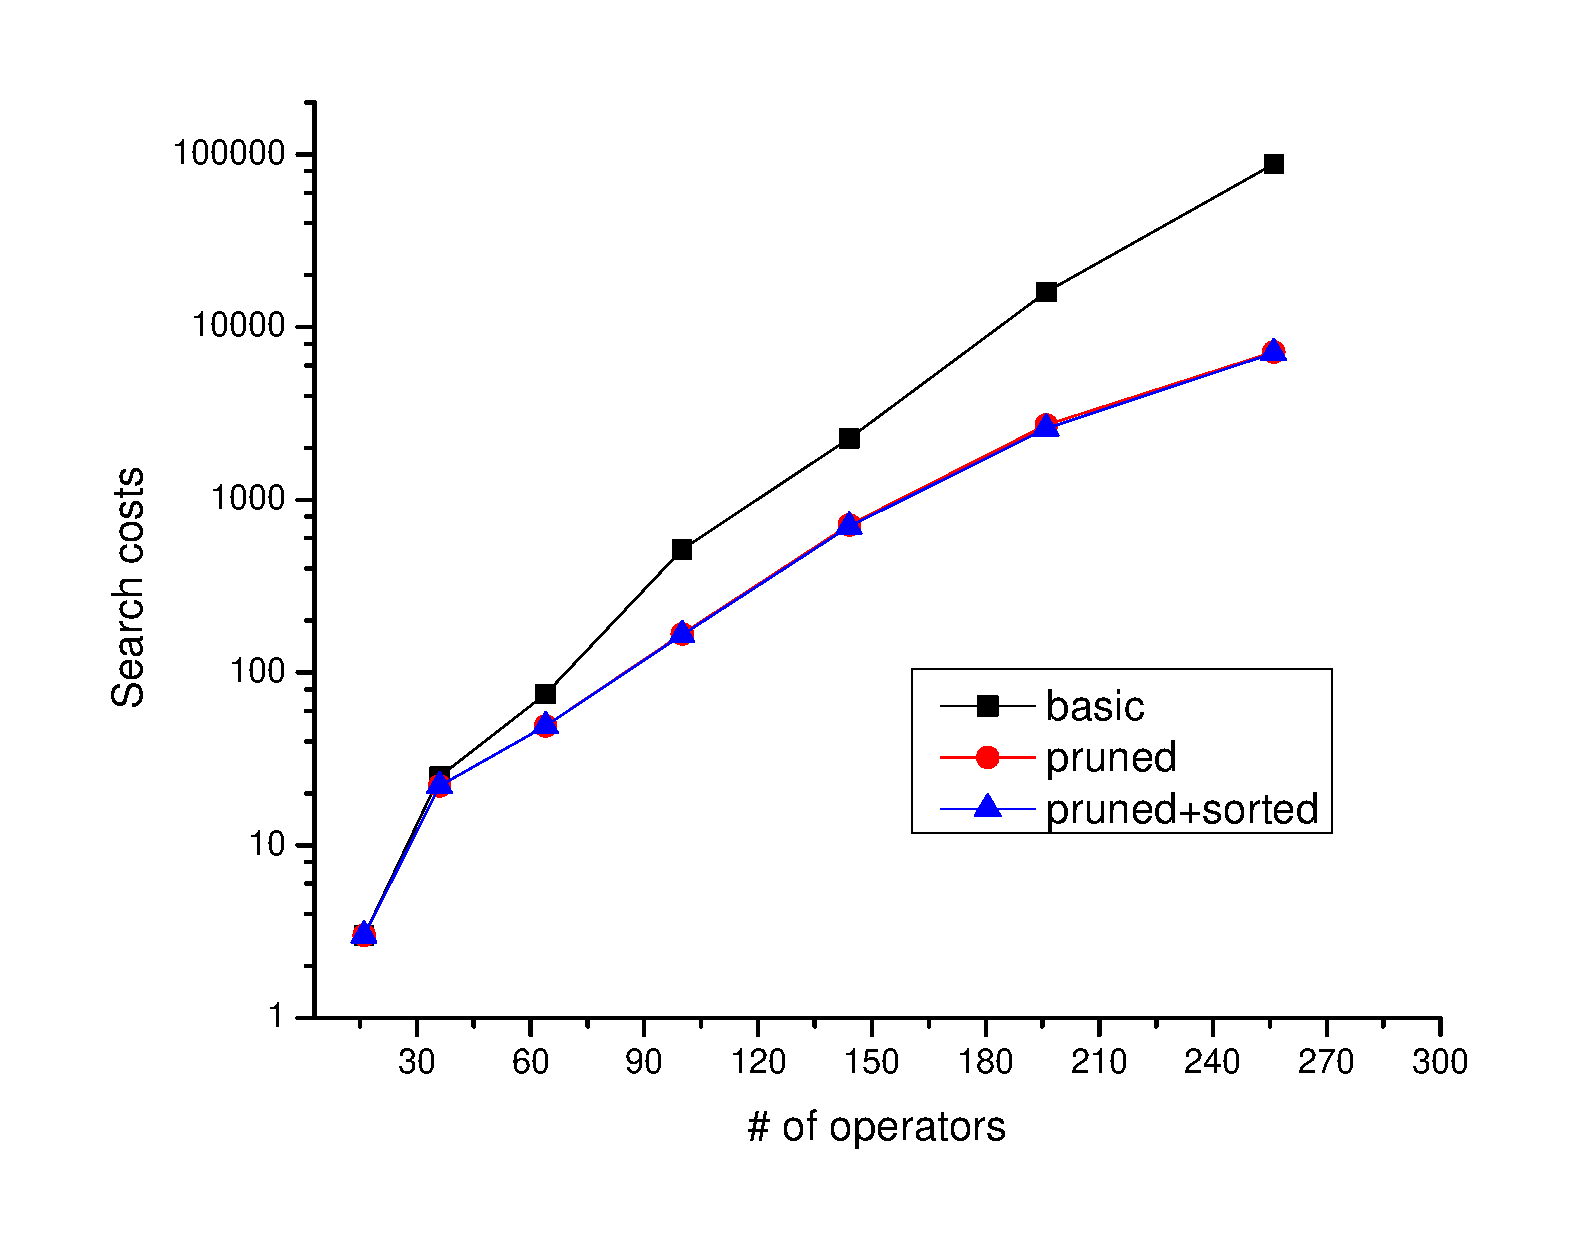
\includegraphics[width=0.324\textwidth]{figures2/eff_rand_num_sample0.5.eps}
\caption{Wrapped figure}
\label{fig:perf}
\end{wrapfigure}

\ifdefined\TTUT
\begin{figure}[!ht]
\begin{center}
    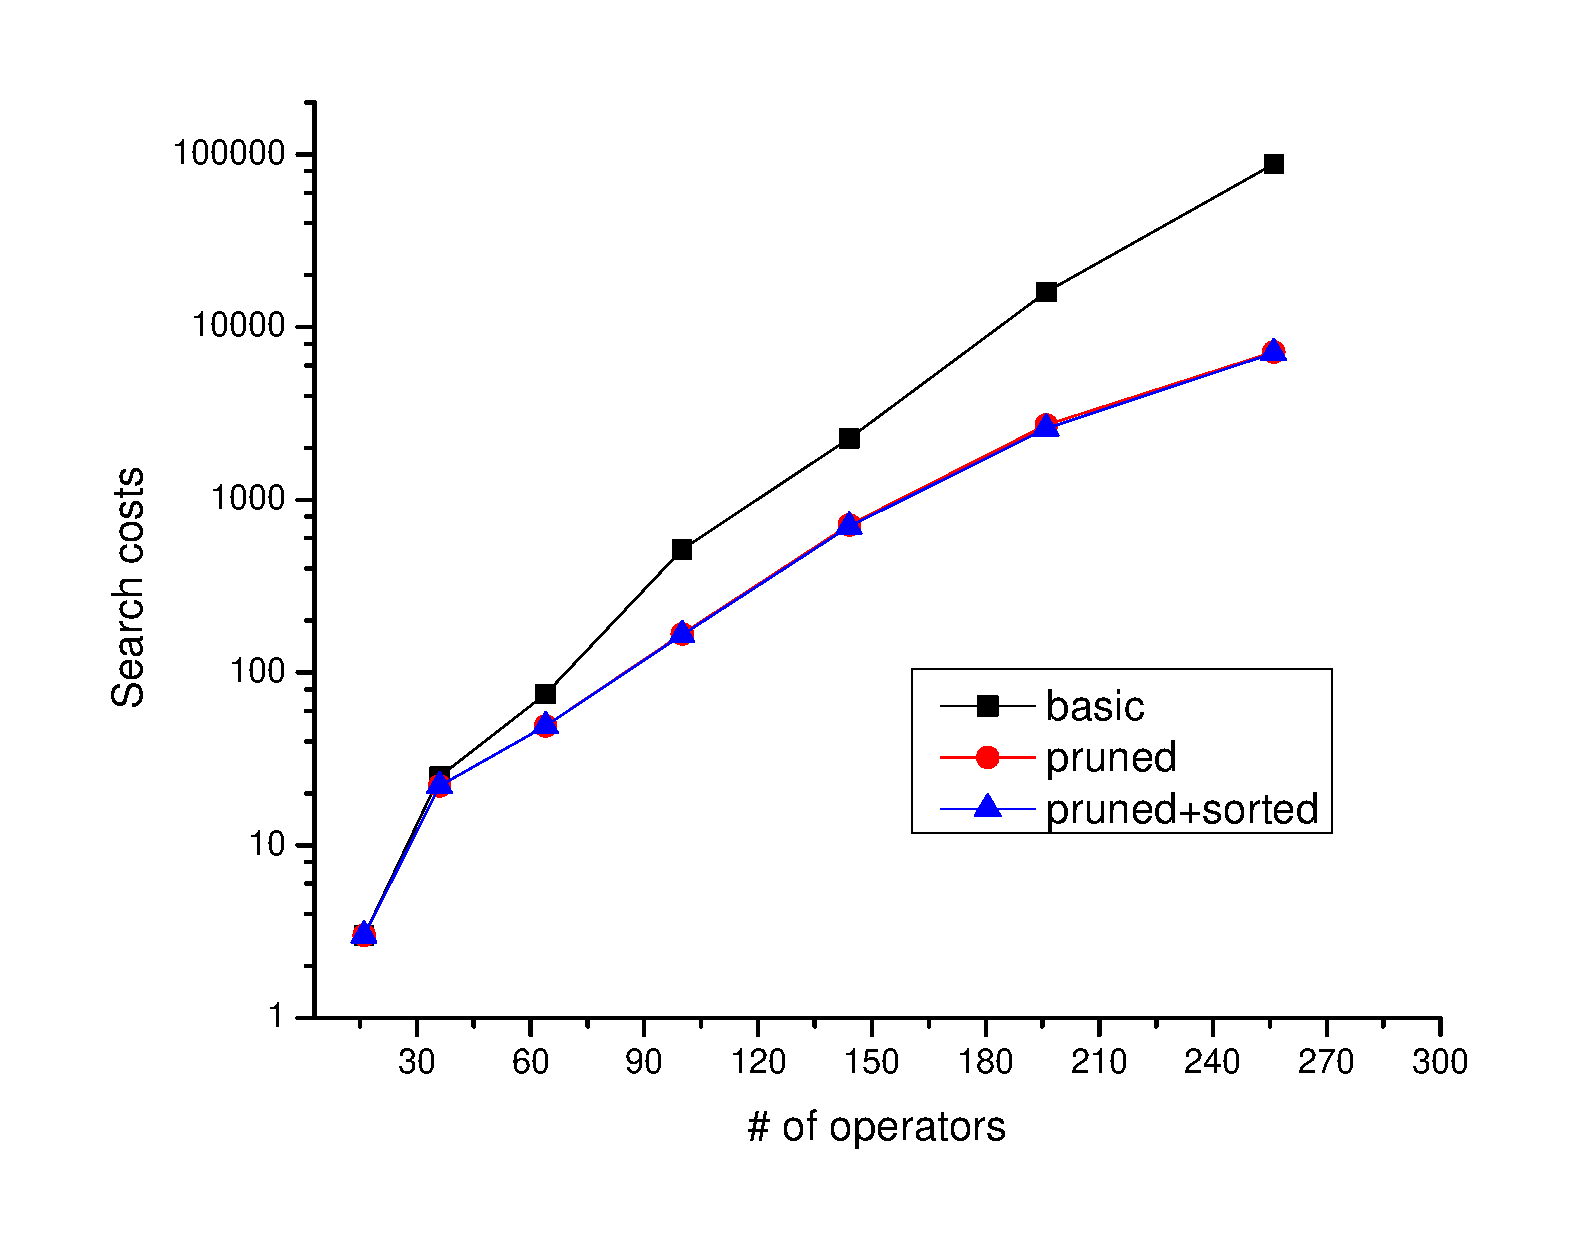
\includegraphics[angle=90, width=0.45\textwidth]{figures2/eff_rand_num_sample0.5.eps}%
\end{center}
%\vspace{-0.15in}
\caption{Easy figure}\label{fig:easy}
\vspace{-0.10in}\end{figure}

\begin{figure*}[!ht]
  \begin{center}
  %\goodgap
    \subfloat[Rotated]{%
      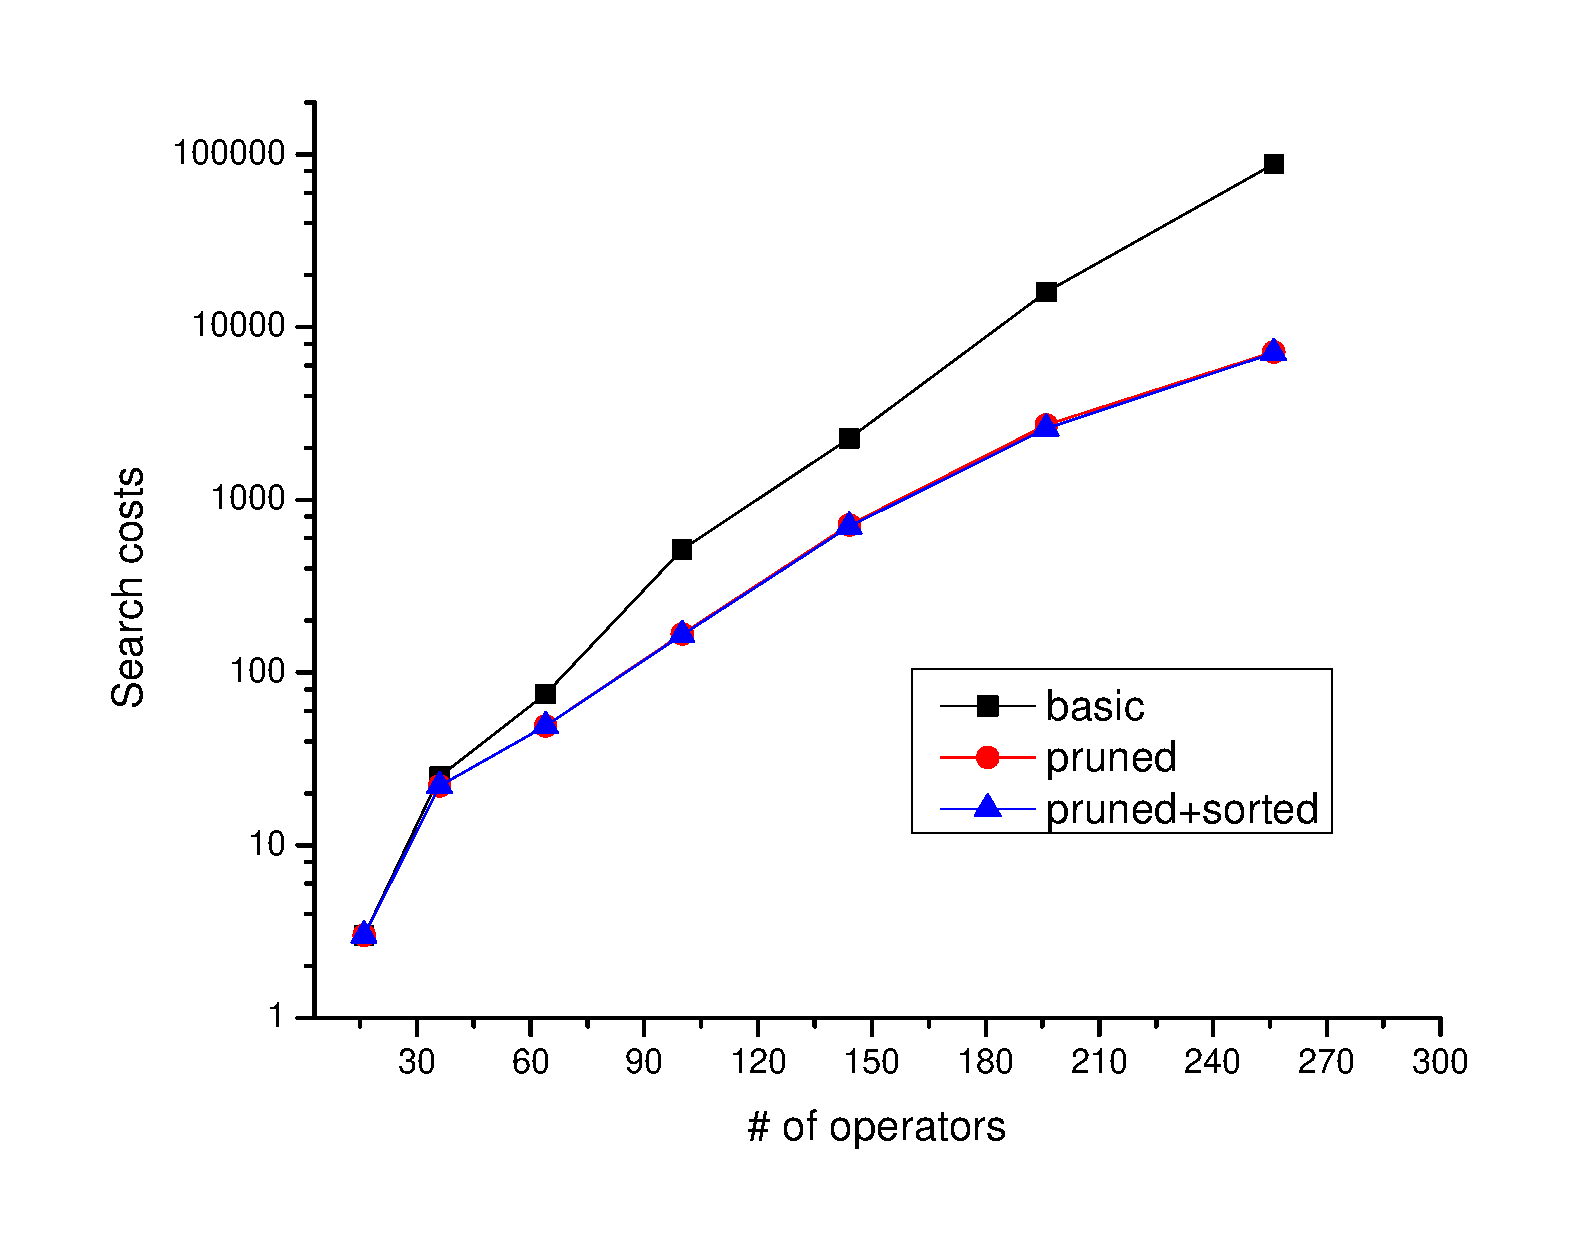
\includegraphics[angle=90, width=0.3\textwidth]{figures2/eff_rand_num_sample0.5.eps}%
      \label{exp:rand_num_1}%
    }%
    %\hspace{-0.2cm}%
    \subfloat[With more shared threads]{%
      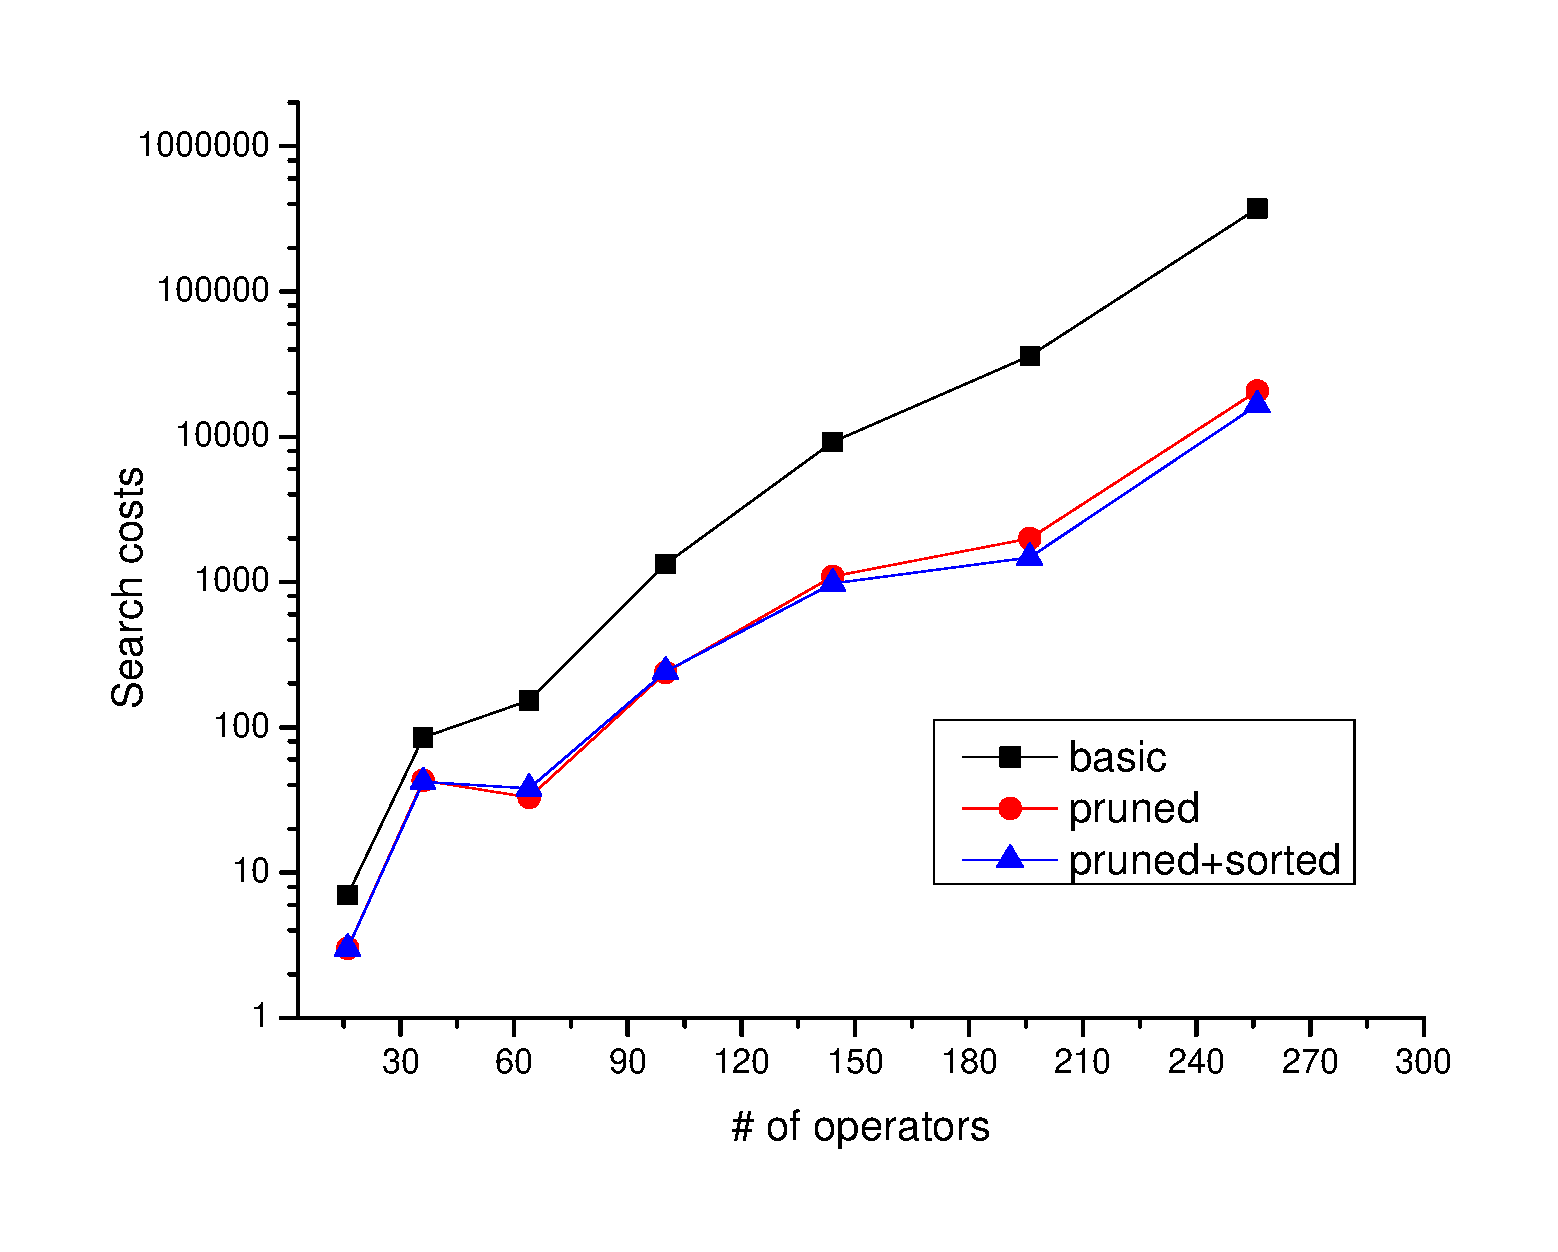
\includegraphics[width=0.3\textwidth]{figures2/eff_rand_num_sample2.eps}%
      \label{exp:rand_num_2}%
    }%
    \subfloat[With sample ratio]{%
      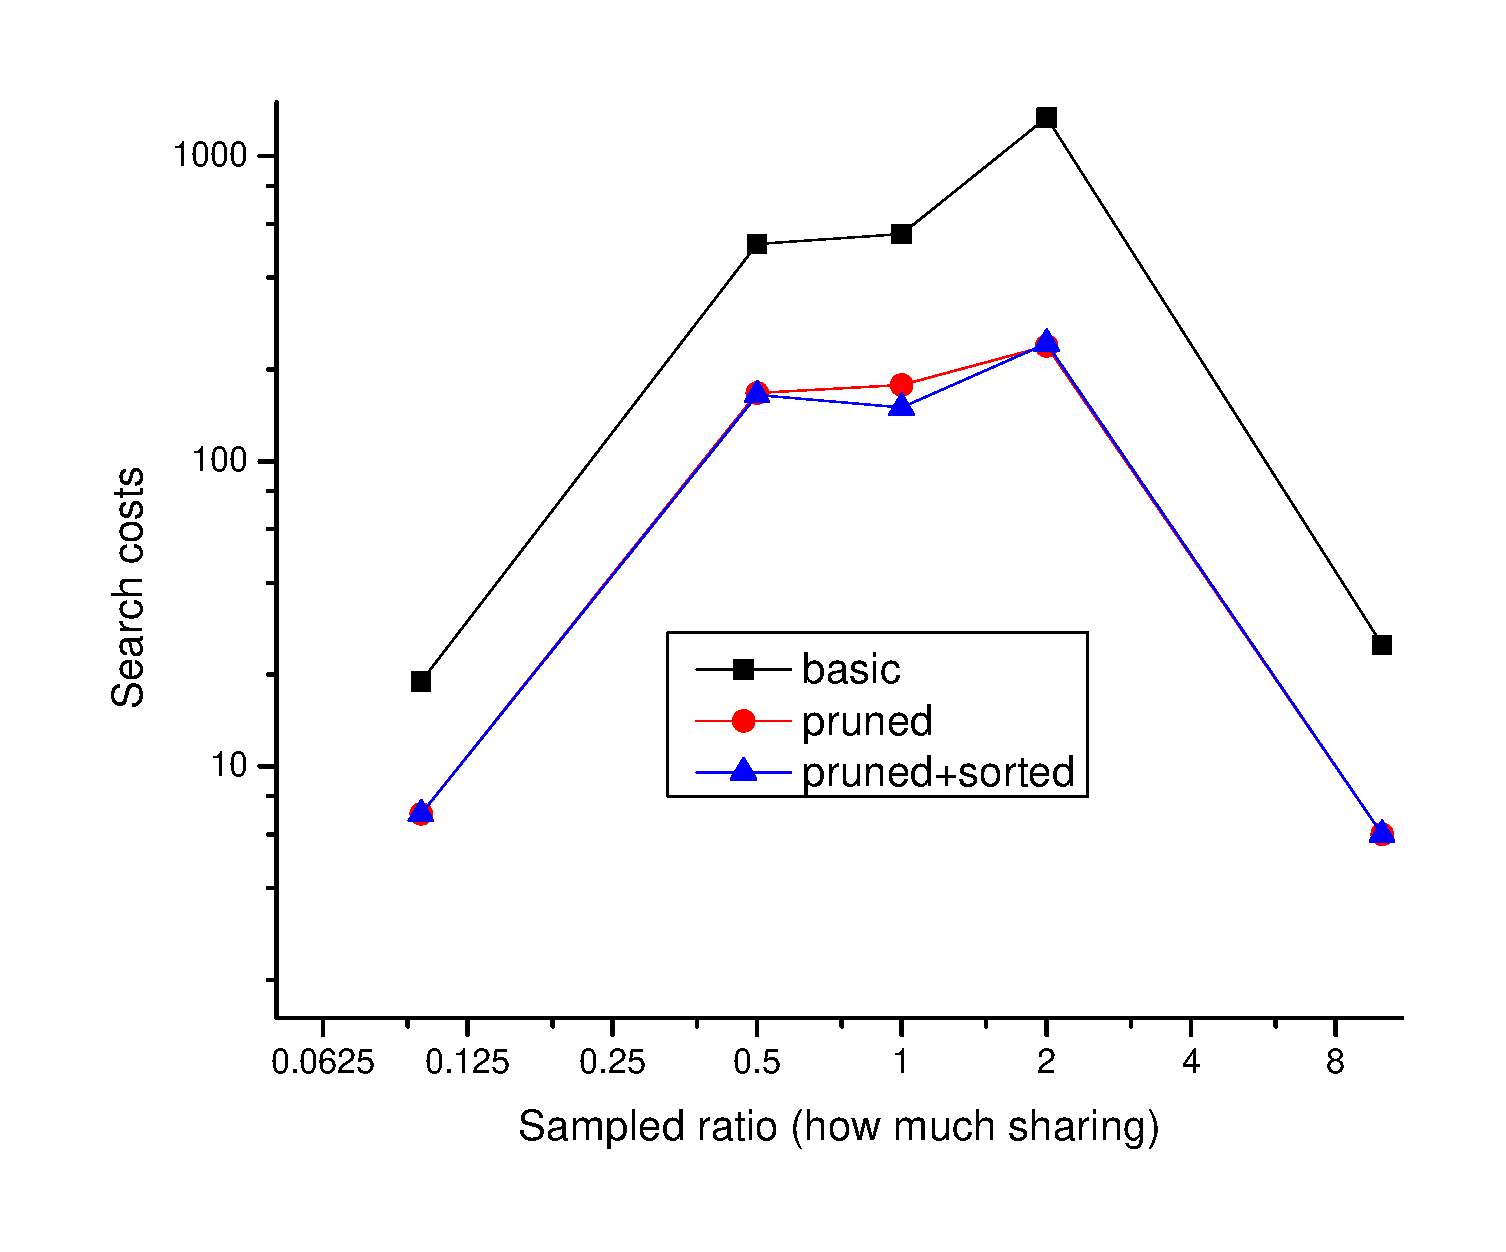
\includegraphics[width=0.3\textwidth]{figures2/eff_rand_sample_num10.eps}%
      \label{exp:rand_sample}%
    }%
  \end{center}%\vspace{-0.15in}
  \caption{Performance of optimization algorithm with random graph}\label{fig:complex}\vspace{-0.10in}
\end{figure*}
\fi

\subsection{algorithms}
\begin{algorithm}[h]
\caption{range-query(range $R$)}\small \label{alg:rangequery}
\begin{algorithmic}[1]
  \boldnext\State $\omega_R\leftarrow $ lowest-common-ancestor($R$) \Comment{comments: line number boldened}
  \State $\lambda\leftarrow $ DHT-lookup($f_{md}(\omega_R)$)
  \ForAll{$p \in P$} \Comment{comments: loop over all items}
    \State manipulate each term $p$
  \EndFor
  \If{$\lambda == NULL \And 1 \leq 0$}
      \State \Return lookup($R$.top\_left\_corner)
  \ElsIf{$R\subseteq{\lambda}$}
      \State \Return the keys of $\lambda$ that are in the range $R$
  \Else
      \State \Return recursive-forward($R$, $\omega_R$)
  \EndIf
\end{algorithmic}
\end{algorithm}

\subsection{equations}
\begin{eqnarray}
u &=& \sum_{l=0}^{n-1}{u_l} \mod{q} %\nonumber \\
=(\sum_{l=0}^{n-1}{ \sum_{j=0}^{c-1}{u_{l-j, j}} \mod{q}})\mod{q} \nonumber \\
&=& (\sum_{j=0}^{c-1}{ \sum_{l=0}^{n-1}{ u_{l-j, j} } })\mod{q} %\nonumber \\
=(\sum_{j=0}^{c-1}{ \sum_{i=-j}^{n-1-j}{ u_{i, j} } })\mod{q} \nonumber \\
&=& (\sum_{j=0}^{c-1}{\sum_{i=0}^{n-1}{ u_{i, j} } }) mod q
= (\sum_{i=0}^{n-1}{ \sum_{j=0}^{c-1}{ u_{i, j} }\mod{q} })\mod{q} \nonumber \\
&=& \sum_{i=0}^{n-1}{ v_i }\mod{q} = \sum_{i=0}^{n-1}{ v_i } = v
\end{eqnarray}

With right brace
\begin{eqnarray}
\underline{\sigma}, \epsilon \rightarrow{}\underline{\beta_*}
\begin{cases}
\begin{rcases}
\begin{rcases}
& \sum_{\forall\beta_*>1}{(\beta_* - 1)} \\
& \sum_{\forall\beta_*<1}{(1 - \beta_*)} \\  
\end{rcases} \rightarrow{} \underline{X_1}\% \\
\sum_{\beta_*<1}{1} \rightarrow{} \underline{X_2}\%
\end{rcases}
\end{cases}
 \rightarrow{\beta}
\end{eqnarray}

\subsection{listing}
\lstset{language=SQL, style=Oracle, caption={Rewritten query against a single view table},label=sql:rewritten}
\lstset{frame=lrbt,xleftmargin=\fboxsep,xrightmargin=-\fboxsep} %with bounding box at l(eft)r(right)b(ottom)t(op)
%or you can replace it with "frame=single"
\begin{lstlisting}
  SELECT A, C FROM viewtable
  ORDER BY C LIMIT arg.k
\end{lstlisting}

\definecolor{mygreen}{rgb}{0,0.6,0}
\begin{figure}[h!]
%\begin{scriptsize}
%\begin{tabular}{cc}
%\begin{minipage}{.5\textwidth}
\lstset{ %
  backgroundcolor=\color{white},   % choose the background color; you must add \usepackage{color} or \usepackage{xcolor}
  %basicstyle=\footnotesize\ttfamily,        % the size of the fonts that are used for the code
  basicstyle=\scriptsize\ttfamily,        % the size of the fonts that are used for the code
  breakatwhitespace=false,         % sets if automatic breaks should only happen at whitespace
  breaklines=true,                 % sets automatic line breaking
  captionpos=b,                    % sets the caption-position to bottom
  commentstyle=\color{mygreen},    % comment style
  deletekeywords={...},            % if you want to delete keywords from the given language
  escapeinside={(*}{*)},          % if you want to add LaTeX within your code
  extendedchars=true,              % lets you use non-ASCII characters; for 8-bits encodings only, does not work with UTF-8
  %frame=single,                    % adds a frame around the code
  keepspaces=true,                 % keeps spaces in text, useful for keeping indentation of code (possibly needs columns=flexible)
  keywordstyle=\color{blue},       % keyword style
  language=Java,                 % the language of the code
  morekeywords={*,...},            % if you want to add more keywords to the set
  numbers=left,                    % where to put the line-numbers; possible values are (none, left, right)
  numbersep=5pt,                   % how far the line-numbers are from the code
  numberstyle=\scriptsize\color{black}, % the style that is used for the line-numbers
  rulecolor=\color{black},         % if not set, the frame-color may be changed on line-breaks within not-black text (e.g. comments (green here))
  showspaces=false,                % show spaces everywhere adding particular underscores; it overrides 'showstringspaces'
  showstringspaces=false,          % underline spaces within strings only
  showtabs=false,                  % show tabs within strings adding particular underscores
  stepnumber=1,                    % the step between two line-numbers. If it's 1, each line will be numbered
  stringstyle=\color{mymauve},     % string literal style
  tabsize=2,                       % sets default tabsize to 2 spaces
  title=\lstname,                  % show the filename of files included with \lstinputlisting; also try caption instead of title
  moredelim=[is][\bf]{*}{*},
}
\begin{lstlisting}
public void OnTouchEvent(MotionEvent e) {
Bitmap LoadPicture(String path) {
    ...
    *Bitmap bm = BitmapFactory.decodeFile(file)*;
    return bm;
}

void EditPicture(Bitmap bm) {
    //heavy computational picture editing
    int i = 10 (* $*$ *); //escape to plot * literatelly instead of bolden text
    bm.getPixels(pix, 0, mPhotoWidth, 0, 0, mPhotoWidth, mPhotoHeight);
    for(every pixel) {
      ...
    }  
    
    //embed location information into picture
    (* $*$*)Location loc = getLastKnownLocation(Provider)*;
    (* $*$*)double longitude = loc.getLongitude()*;
    (* $*$*)double latitude = loc.getLatitude()*;
    (* $*$*)EmbedLocation(bm, longitude, latitude);*
}
\end{lstlisting}
%\end{minipage}
%\end{tabular}
%\end{scriptsize}
\caption{Privacy-preserving Offloading Example}
\label{figure:MotivatingExample}
\end{figure}


\subsection{fbox}
\begin{center}
\fbox{This is a sample statement}
\end{center}

\begin{center}
\fbox{\parbox{0.90\linewidth}{
This is a long long long statement: 
Blah blah blah blah 
Blah blah blah blah 
Blah blah blah blah 
Blah blah blah blah 
Blah blah blah blah 
Blah blah blah blah 
Blah blah blah blah 
Blah blah blah blah 
}}
\end{center}



\subsection{misc}
\begin{itemize}
  \item caret $\textrm{\^{}}$ 
  \item cmark $\cmark$ and xmark $\xmark$
  \item bold math type $\boldsymbol{<v_0, k>}$
  \item use other than default font size: {``\fontsize{8.5}{9} this's in font size 8.5''}. (second param. should be 1.2$\times$ first param. which is font size
  \item show tilde in url, use \textasciitilde{} rather than \~{}
  \item strike out text, \sout{text/$12$ removed}
  \item color, {\color{red}red}{\color{green}green}
  \item[$\bullet$] big bullet on each item
  \item circled text \circled{2}
  \item A white number inside a black circle: \ballnumber{37}
  \item empty set (beautiful version) $\varnothing$ (needs ``\\usepackage\{amssymb\}''), which renames emptyset, $\emptyset$
  \item stackrel $\stackrel[c]{a}{=}$
\end{itemize}

citation for long breakable url~\cite{me:mssgx}


\fi

\ifdefined\TTTARGETaddontwo
  \providecommand{\ssssp}{{\sc SS\_SSP}\xspace}
\newcommand{\yuzhe}[1]{\footnote{\textcolor{red}{(Yuzhe: #1)}}}

%\input{/Users/tristartom/workspace/teaching/crypto/600-applied_crypto/lecnotes/text/t_crypto_preamble.tex}

\definecolor{mygreen}{rgb}{0,0.6,0}
%
\lstset{ %
  backgroundcolor=\color{white},   % choose the background color; you must add \usepackage{color} or \usepackage{xcolor}
  %basicstyle=\footnotesize\ttfamily,        % the size of the fonts that are used for the code
  basicstyle=\scriptsize\ttfamily,        % the size of the fonts that are used for the code
  breakatwhitespace=false,         % sets if automatic breaks should only happen at whitespace
  breaklines=true,                 % sets automatic line breaking
  captionpos=b,                    % sets the caption-position to bottom
  commentstyle=\color{mygreen},    % comment style
  deletekeywords={...},            % if you want to delete keywords from the given language
  escapeinside={\%*}{*)},          % if you want to add LaTeX within your code
  extendedchars=true,              % lets you use non-ASCII characters; for 8-bits encodings only, does not work with UTF-8
  %frame=single,                    % adds a frame around the code
  keepspaces=true,                 % keeps spaces in text, useful for keeping indentation of code (possibly needs columns=flexible)
  keywordstyle=\color{blue},       % keyword style
  language=Java,                 % the language of the code
  morekeywords={*,...},            % if you want to add more keywords to the set
  numbers=left,                    % where to put the line-numbers; possible values are (none, left, right)
  numbersep=5pt,                   % how far the line-numbers are from the code
  numberstyle=\scriptsize\color{black}, % the style that is used for the line-numbers
  rulecolor=\color{black},         % if not set, the frame-color may be changed on line-breaks within not-black text (e.g. comments (green here))
  showspaces=false,                % show spaces everywhere adding particular underscores; it overrides 'showstringspaces'
  showstringspaces=false,          % underline spaces within strings only
  showtabs=false,                  % show tabs within strings adding particular underscores
  stepnumber=1,                    % the step between two line-numbers. If it's 1, each line will be numbered
  stringstyle=\color{mymauve},     % string literal style
  tabsize=2,                       % sets default tabsize to 2 spaces
  title=\lstname,                  % show the filename of files included with \lstinputlisting; also try caption instead of title
  moredelim=[is][\bf]{*}{*},
}

\tableofcontents
\newpage

\ifdefined\TTSTYLETARGETreport
\chapter{Ch 1 (only in report mode)}
\chapter{Ch 2 (only in report mode)}
\fi

Prior work, Prior work, Prior work~\tangSide{test content}.


\section{Overview} \label{sec:overview}
\section{Main Body} \label{sec:mainbody}
Prior work~\cite{DBLP:books/crc/KatzLindell2007}

we propose {\ssssp}.

\url{www.cc.gatech.edu/~ytang36/}

\newpage
\newpage


\clearpage
\section{learning}

\begin{theorem}
\end{theorem}
\begin{proof}
\end{proof}

\subsection{tables}

{\scriptsize \begin{verbatim} in beamer, see beamer_learn_slides. http://en.wikibooks.org/wiki/LaTeX/Tables#The_tabular.2A_environment_-_controlling_table_width
\end{verbatim}}

table with reference~\ref{tab:auth-attack}


\begin{table*}[!htbp] %force in current page, disable float.
\caption{Example of authorized searcher attack}
\label{tab:auth-attack}\centering{\small
\begin{tabularx}{0.5\textwidth}{ |X|c|c|c|c|c| }
  \hline
   & $p_0$ & $p_1$ & $p_2$ & $p_3$ & $p_4$ \\ \hline
  $r_a$ & $1$ & $0$ & $1$ & $0$ & $?$ \\ \hline
\end{tabularx}
}
\end{table*}

tabular (not table)

\begin{tabularx}{0.4\textwidth}{ |X|c|c|c| } %X is stretching to \textwidth, while c is to match with text width in cell.
  \hline
  label1                    & label2 & label3 & label4 \\ \hline
  \multirow{2}{*}{multi-row} 
                             & item2  & item3  & item4  \\ \cline{2-4}
                             & item2'  & item3'  & item4'  \\ \hline
  \multicolumn{2}{|l|}{multi-column}   & item3''  & item4''  \\  \hline
  \multirow{5}{*}{\begin{sideways}sideways\end{sideways}}
                             & item2  & item3  & item4  \\ \cline{2-4}
                             & \shortstack[l]{item2'\\item2''}  & item3'  & item4'  \\ \cline{2-4}
                             & \shortstack[r]{item2'\\item2''}  & item3'  & item4'  \\ \cline{2-4}
                             & item2'  & item3'  & item4'  \\ \cline{2-4}
                             & item2'  & item3'  & item4'  \\ \hline
\end{tabularx}

Table with diagbox

\begin{tabular}{|c|c|}
    \hline
    alghreaiog & bghsah \\
    \hline
    cagja & \notableentry \\
    \hline
    \cellcolor{blue} & edkhaklgjaj \\
    \hline
\end{tabular}

\begin{tabular}{|p{4cm}|p{3cm}|}
    \hline
    alghreaiog & bghsah \\
    \hline
    cagja\par bla & \notableentry \\
    \hline
    \cellcolor{blue} & edkhaklgjaj \par xyz \\
    \hline
\end{tabular}

Table line/cell/column colored

\begin{table}[ht]
\centering
\begin{tabular}{c|ccccccc}
\hline
& col1 & col2 & col3 & col4 & col5 & col6 & col7 \\
\hline
\rowcolor{LightCyan}
row1& \ra & \ra & \ra & \ra & \ra & \ra & \ra \\
row2& \ra & \ra & \ra & \ra & \ra & \ra & \ra \\
\rowcolor{LightCyan}
row3& \ra & \ra & \ra & \ra & \ra & \ra & \ra \\
row4& \ra & \ra & \ra & \ra & \ra & \ra & \ra \\
\rowcolor{LightCyan}
row5& \ra & \ra & \ra & \ra & \ra & \ra & \ra \\
row6& \ra & \ra & \ra & \ra & \ra & \ra & \ra \\
\hline
\end{tabular}
\end{table}

\newcolumntype{g}{>{\columncolor{Gray}}c}
\begin{table}[ht]
\centering
\begin{tabular}{c|g|c|g|c|g|c|g}
\hline
&col1 &col2 &col3 &col4 & col5 &col6 &col7\\
\hline
row1& \ra & \ra & \ra & \ra & \ra & \ra & \ra \\
row2& \ra & \ra & \ra & \ra & \ra & \ra & \ra \\
row3& \ra & \ra & \ra & \ra & \ra & \ra & \ra \\
row4& \ra & \ra & \ra & \ra & \ra & \ra & \ra \\
row5& \ra & \ra & \ra & \ra & \ra & \ra & \ra \\
row6& \ra & \ra & \ra & \ra & \ra & \ra & \ra \\
\hline
\end{tabular}
\end{table}



\subsection{figures}
\begin{wrapfigure}{r}{0.35\textwidth}
\centering
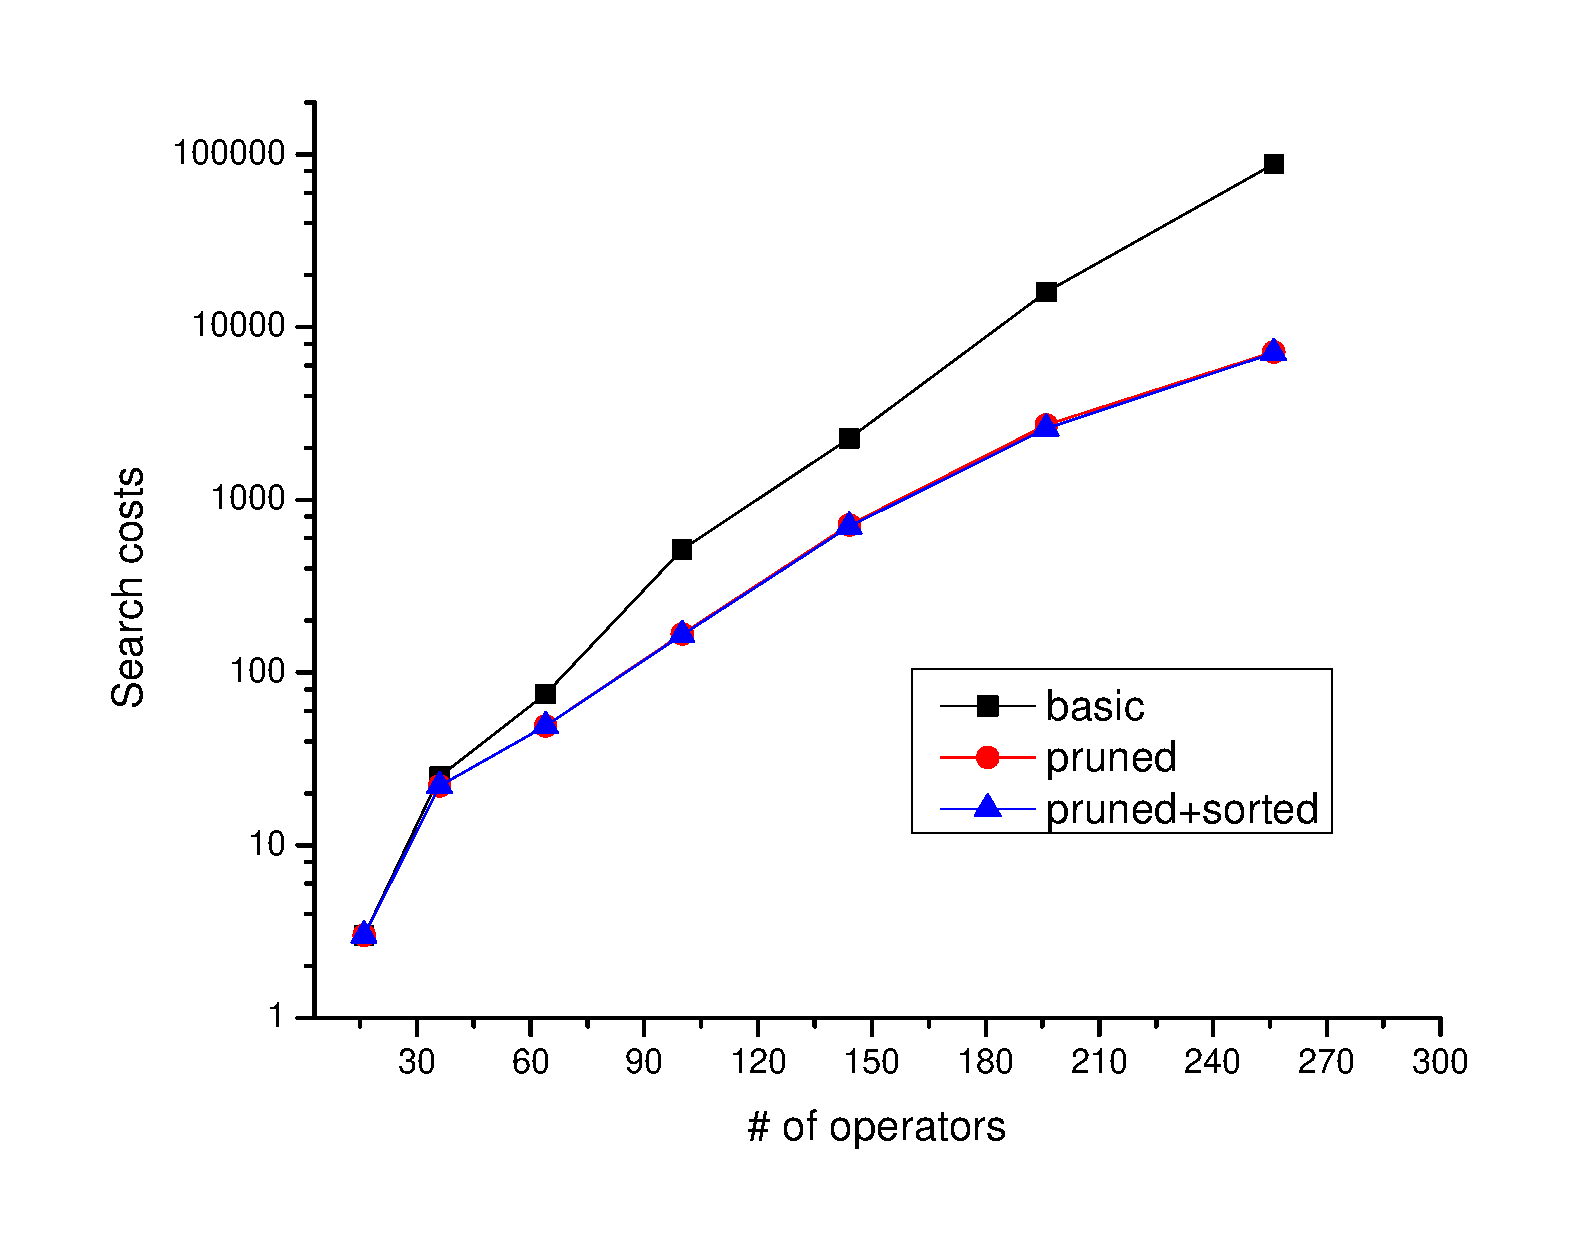
\includegraphics[width=0.324\textwidth]{figures2/eff_rand_num_sample0.5.eps}
\caption{Wrapped figure}
\label{fig:perf}
\end{wrapfigure}

\ifdefined\TTUT
\begin{figure}[!ht]
\begin{center}
    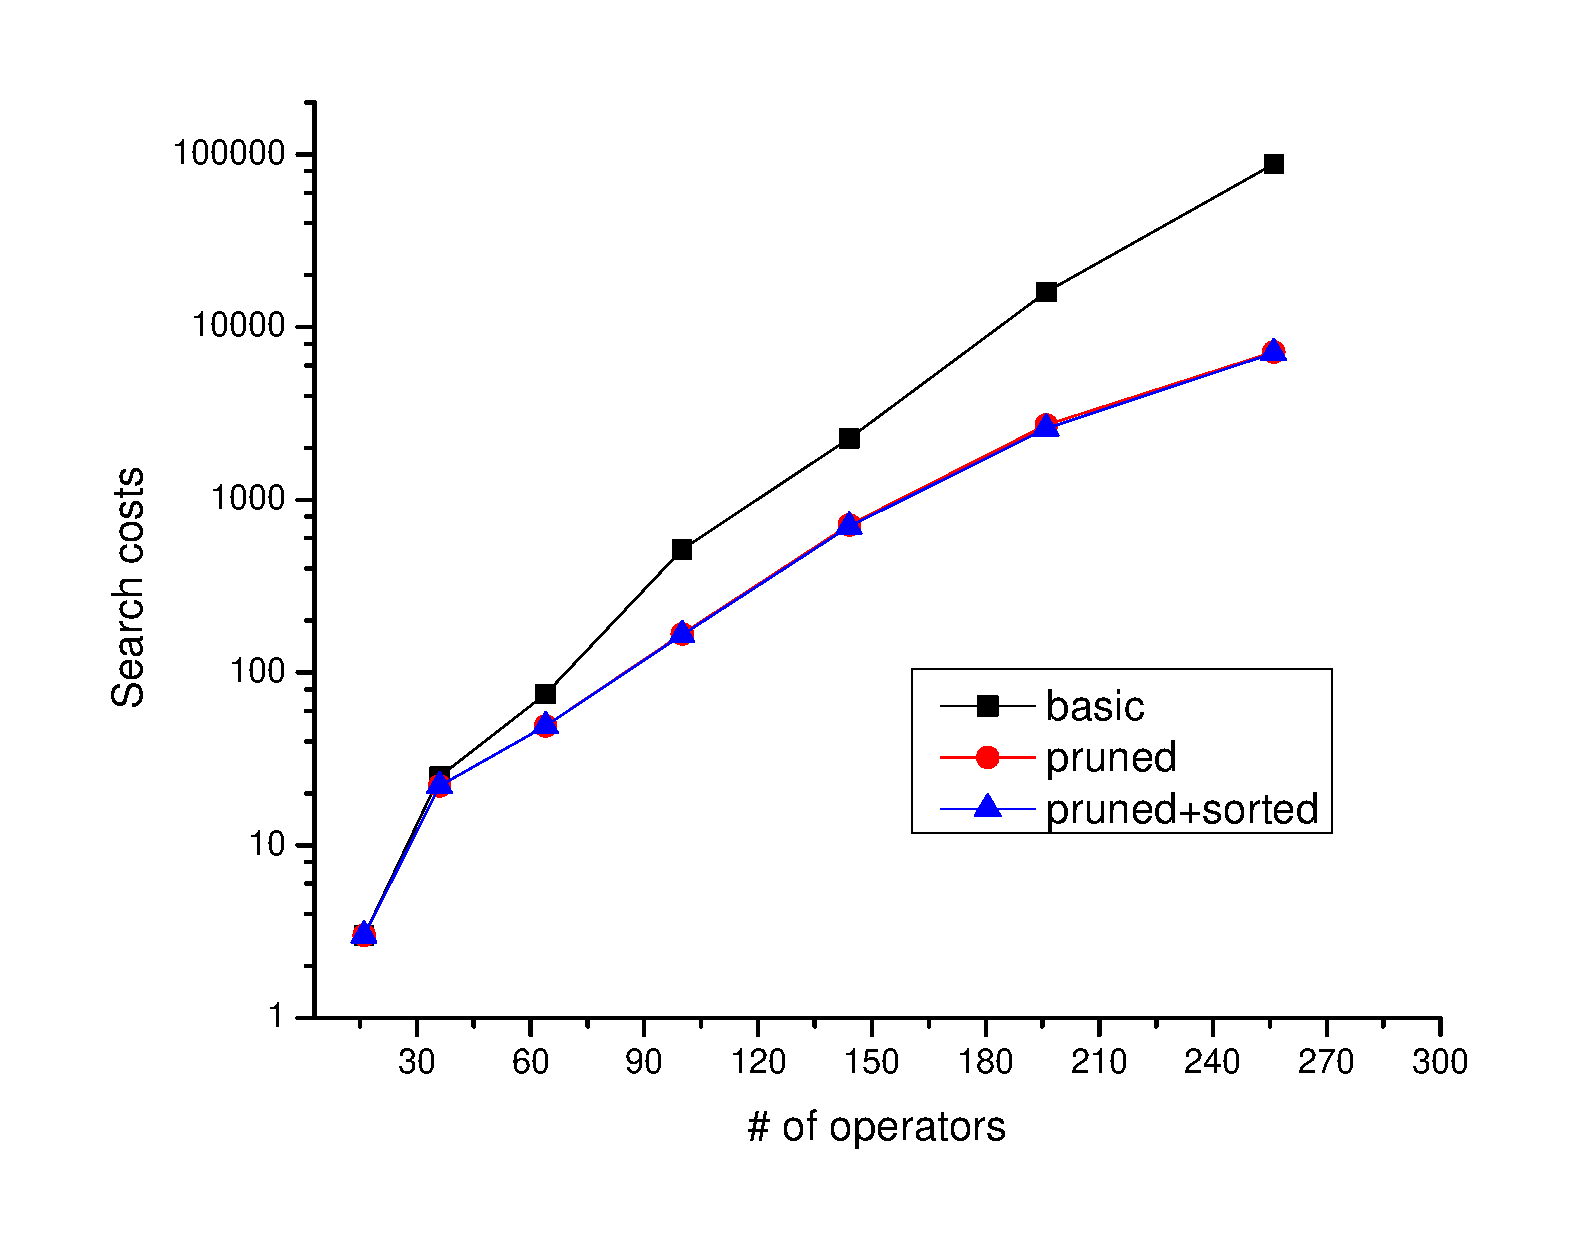
\includegraphics[angle=90, width=0.45\textwidth]{figures2/eff_rand_num_sample0.5.eps}%
\end{center}
%\vspace{-0.15in}
\caption{Easy figure}\label{fig:easy}
\vspace{-0.10in}\end{figure}

\begin{figure*}[!ht]
  \begin{center}
  %\goodgap
    \subfloat[Rotated]{%
      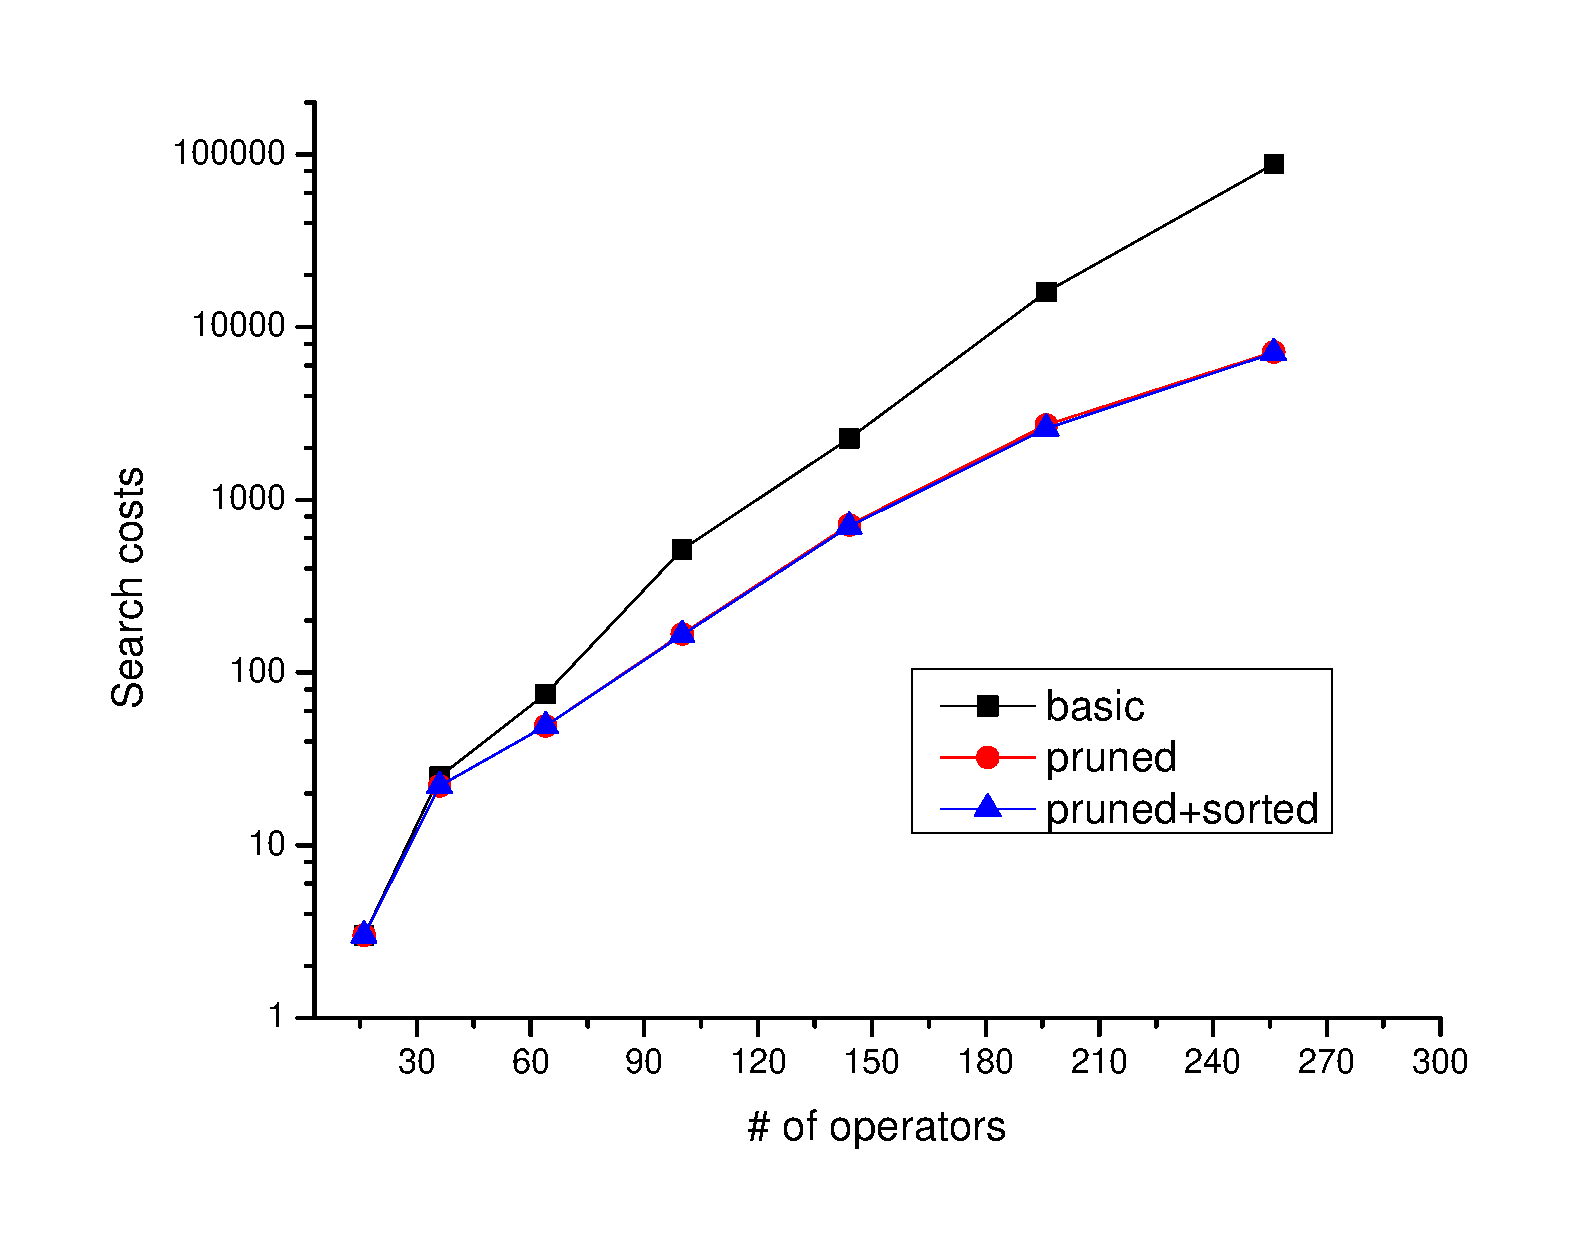
\includegraphics[angle=90, width=0.3\textwidth]{figures2/eff_rand_num_sample0.5.eps}%
      \label{exp:rand_num_1}%
    }%
    %\hspace{-0.2cm}%
    \subfloat[With more shared threads]{%
      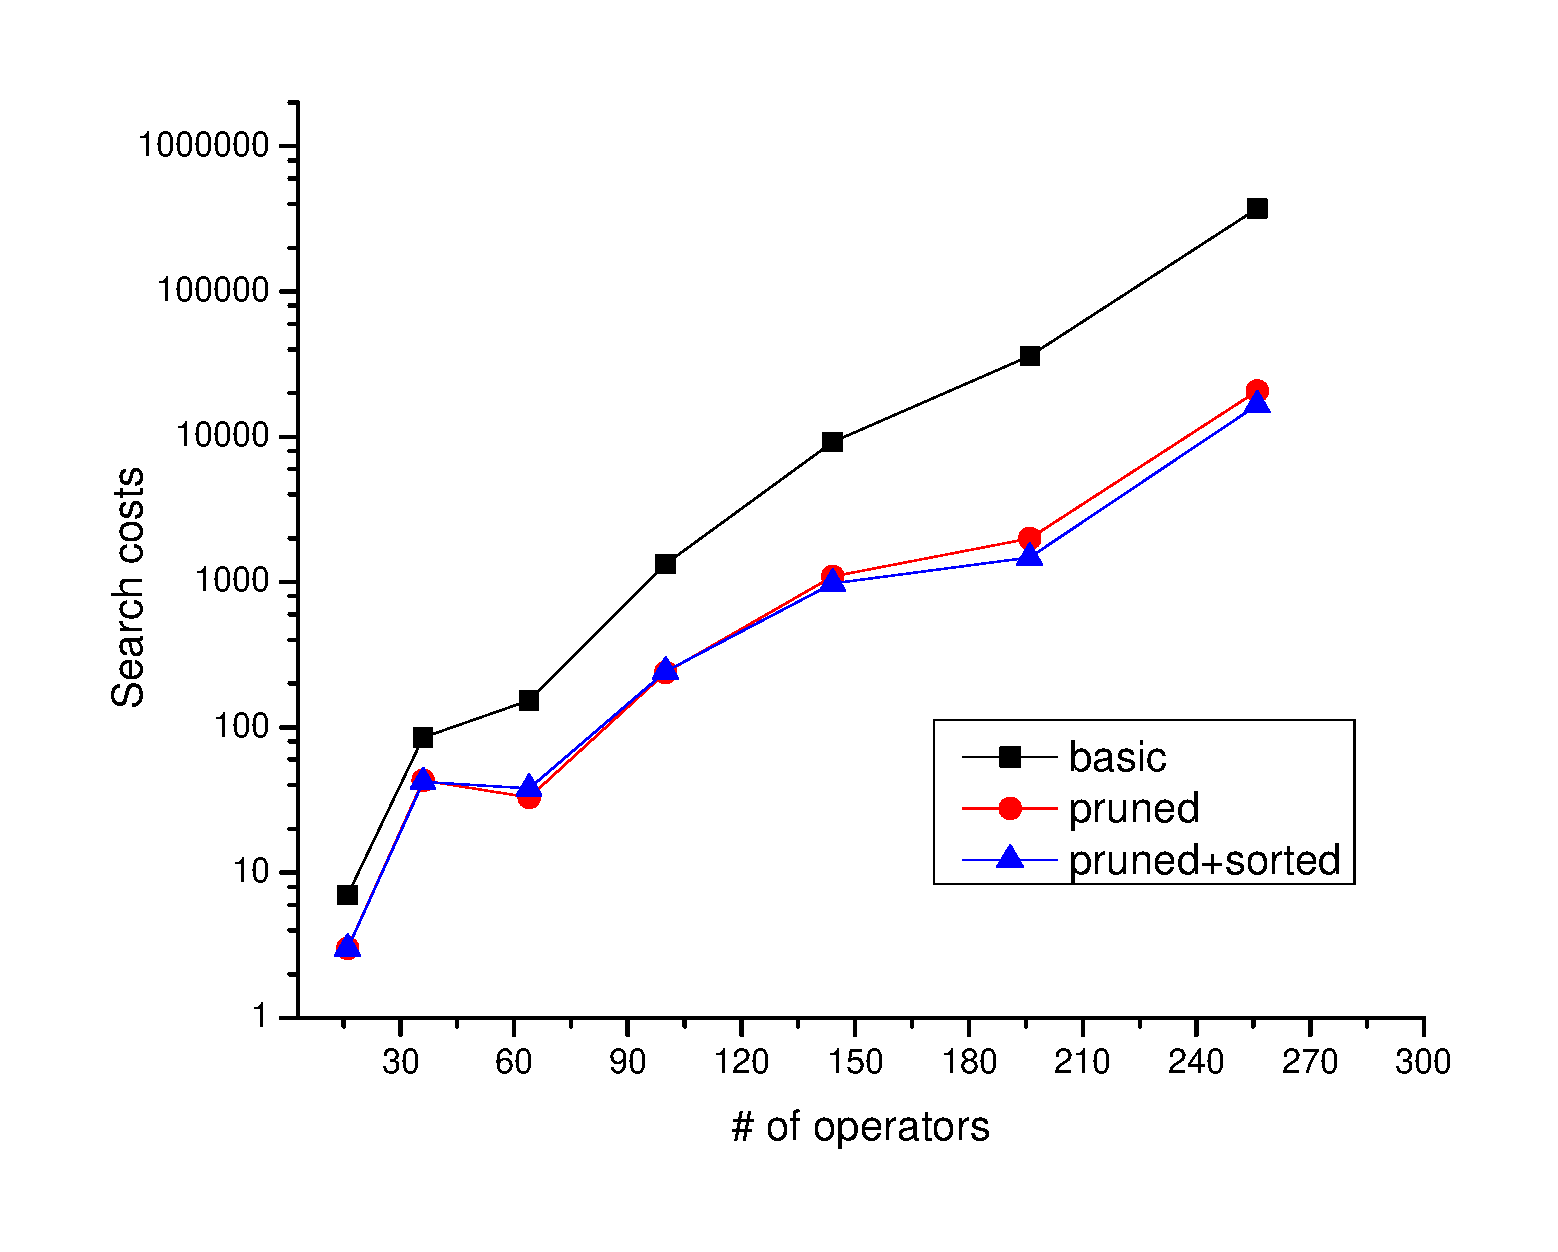
\includegraphics[width=0.3\textwidth]{figures2/eff_rand_num_sample2.eps}%
      \label{exp:rand_num_2}%
    }%
    \subfloat[With sample ratio]{%
      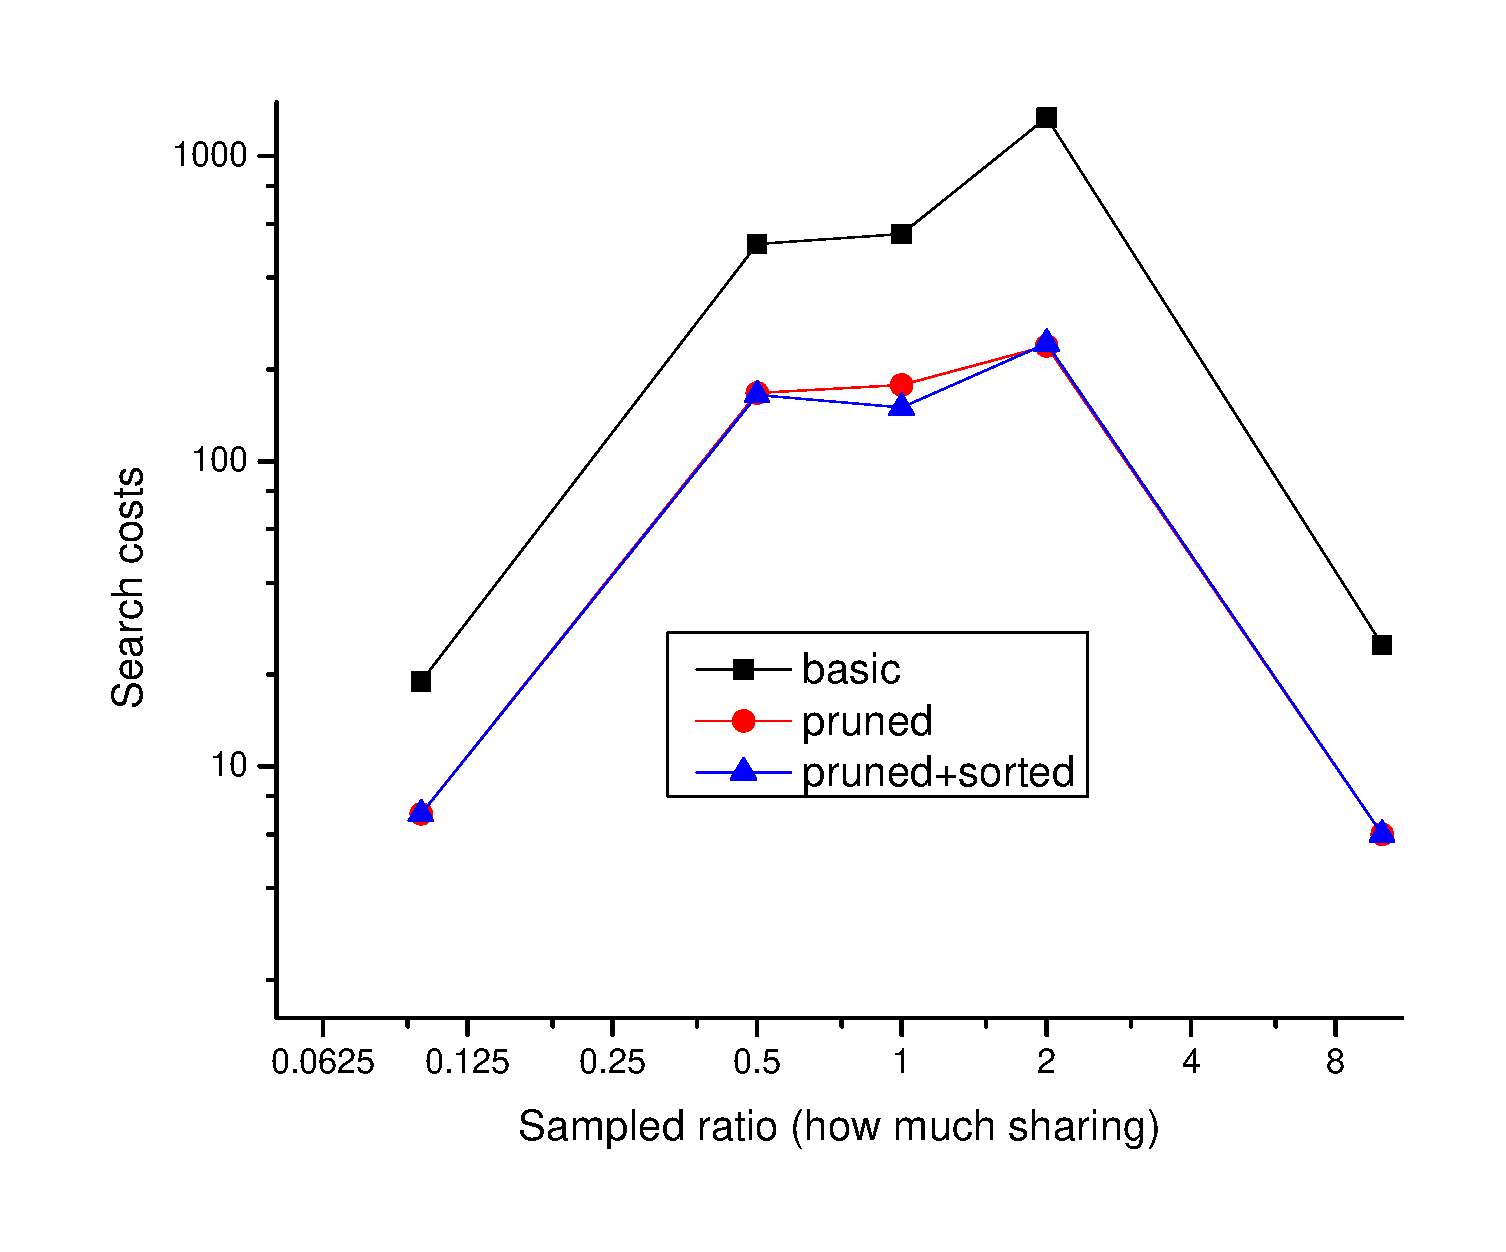
\includegraphics[width=0.3\textwidth]{figures2/eff_rand_sample_num10.eps}%
      \label{exp:rand_sample}%
    }%
  \end{center}%\vspace{-0.15in}
  \caption{Performance of optimization algorithm with random graph}\label{fig:complex}\vspace{-0.10in}
\end{figure*}
\fi

\subsection{algorithms}
\begin{algorithm}[h]
\caption{range-query(range $R$)}\small \label{alg:rangequery}
\begin{algorithmic}[1]
  \boldnext\State $\omega_R\leftarrow $ lowest-common-ancestor($R$) \Comment{comments: line number boldened}
  \State $\lambda\leftarrow $ DHT-lookup($f_{md}(\omega_R)$)
  \ForAll{$p \in P$} \Comment{comments: loop over all items}
    \State manipulate each term $p$
  \EndFor
  \If{$\lambda == NULL \And 1 \leq 0$}
      \State \Return lookup($R$.top\_left\_corner)
  \ElsIf{$R\subseteq{\lambda}$}
      \State \Return the keys of $\lambda$ that are in the range $R$
  \Else
      \State \Return recursive-forward($R$, $\omega_R$)
  \EndIf
\end{algorithmic}
\end{algorithm}

\subsection{equations}
\begin{eqnarray}
u &=& \sum_{l=0}^{n-1}{u_l} \mod{q} %\nonumber \\
=(\sum_{l=0}^{n-1}{ \sum_{j=0}^{c-1}{u_{l-j, j}} \mod{q}})\mod{q} \nonumber \\
&=& (\sum_{j=0}^{c-1}{ \sum_{l=0}^{n-1}{ u_{l-j, j} } })\mod{q} %\nonumber \\
=(\sum_{j=0}^{c-1}{ \sum_{i=-j}^{n-1-j}{ u_{i, j} } })\mod{q} \nonumber \\
&=& (\sum_{j=0}^{c-1}{\sum_{i=0}^{n-1}{ u_{i, j} } }) mod q
= (\sum_{i=0}^{n-1}{ \sum_{j=0}^{c-1}{ u_{i, j} }\mod{q} })\mod{q} \nonumber \\
&=& \sum_{i=0}^{n-1}{ v_i }\mod{q} = \sum_{i=0}^{n-1}{ v_i } = v
\end{eqnarray}

With right brace
\begin{eqnarray}
\underline{\sigma}, \epsilon \rightarrow{}\underline{\beta_*}
\begin{cases}
\begin{rcases}
\begin{rcases}
& \sum_{\forall\beta_*>1}{(\beta_* - 1)} \\
& \sum_{\forall\beta_*<1}{(1 - \beta_*)} \\  
\end{rcases} \rightarrow{} \underline{X_1}\% \\
\sum_{\beta_*<1}{1} \rightarrow{} \underline{X_2}\%
\end{rcases}
\end{cases}
 \rightarrow{\beta}
\end{eqnarray}

\subsection{listing}
\lstset{language=SQL, style=Oracle, caption={Rewritten query against a single view table},label=sql:rewritten}
\lstset{frame=lrbt,xleftmargin=\fboxsep,xrightmargin=-\fboxsep} %with bounding box at l(eft)r(right)b(ottom)t(op)
%or you can replace it with "frame=single"
\begin{lstlisting}
  SELECT A, C FROM viewtable
  ORDER BY C LIMIT arg.k
\end{lstlisting}

\definecolor{mygreen}{rgb}{0,0.6,0}
\begin{figure}[h!]
%\begin{scriptsize}
%\begin{tabular}{cc}
%\begin{minipage}{.5\textwidth}
\lstset{ %
  backgroundcolor=\color{white},   % choose the background color; you must add \usepackage{color} or \usepackage{xcolor}
  %basicstyle=\footnotesize\ttfamily,        % the size of the fonts that are used for the code
  basicstyle=\scriptsize\ttfamily,        % the size of the fonts that are used for the code
  breakatwhitespace=false,         % sets if automatic breaks should only happen at whitespace
  breaklines=true,                 % sets automatic line breaking
  captionpos=b,                    % sets the caption-position to bottom
  commentstyle=\color{mygreen},    % comment style
  deletekeywords={...},            % if you want to delete keywords from the given language
  escapeinside={(*}{*)},          % if you want to add LaTeX within your code
  extendedchars=true,              % lets you use non-ASCII characters; for 8-bits encodings only, does not work with UTF-8
  %frame=single,                    % adds a frame around the code
  keepspaces=true,                 % keeps spaces in text, useful for keeping indentation of code (possibly needs columns=flexible)
  keywordstyle=\color{blue},       % keyword style
  language=Java,                 % the language of the code
  morekeywords={*,...},            % if you want to add more keywords to the set
  numbers=left,                    % where to put the line-numbers; possible values are (none, left, right)
  numbersep=5pt,                   % how far the line-numbers are from the code
  numberstyle=\scriptsize\color{black}, % the style that is used for the line-numbers
  rulecolor=\color{black},         % if not set, the frame-color may be changed on line-breaks within not-black text (e.g. comments (green here))
  showspaces=false,                % show spaces everywhere adding particular underscores; it overrides 'showstringspaces'
  showstringspaces=false,          % underline spaces within strings only
  showtabs=false,                  % show tabs within strings adding particular underscores
  stepnumber=1,                    % the step between two line-numbers. If it's 1, each line will be numbered
  stringstyle=\color{mymauve},     % string literal style
  tabsize=2,                       % sets default tabsize to 2 spaces
  title=\lstname,                  % show the filename of files included with \lstinputlisting; also try caption instead of title
  moredelim=[is][\bf]{*}{*},
}
\begin{lstlisting}
public void OnTouchEvent(MotionEvent e) {
Bitmap LoadPicture(String path) {
    ...
    *Bitmap bm = BitmapFactory.decodeFile(file)*;
    return bm;
}

void EditPicture(Bitmap bm) {
    //heavy computational picture editing
    int i = 10 (* $*$ *); //escape to plot * literatelly instead of bolden text
    bm.getPixels(pix, 0, mPhotoWidth, 0, 0, mPhotoWidth, mPhotoHeight);
    for(every pixel) {
      ...
    }  
    
    //embed location information into picture
    (* $*$*)Location loc = getLastKnownLocation(Provider)*;
    (* $*$*)double longitude = loc.getLongitude()*;
    (* $*$*)double latitude = loc.getLatitude()*;
    (* $*$*)EmbedLocation(bm, longitude, latitude);*
}
\end{lstlisting}
%\end{minipage}
%\end{tabular}
%\end{scriptsize}
\caption{Privacy-preserving Offloading Example}
\label{figure:MotivatingExample}
\end{figure}


\subsection{fbox}
\begin{center}
\fbox{This is a sample statement}
\end{center}

\begin{center}
\fbox{\parbox{0.90\linewidth}{
This is a long long long statement: 
Blah blah blah blah 
Blah blah blah blah 
Blah blah blah blah 
Blah blah blah blah 
Blah blah blah blah 
Blah blah blah blah 
Blah blah blah blah 
Blah blah blah blah 
}}
\end{center}



\subsection{misc}
\begin{itemize}
  \item caret $\textrm{\^{}}$ 
  \item cmark $\cmark$ and xmark $\xmark$
  \item bold math type $\boldsymbol{<v_0, k>}$
  \item use other than default font size: {``\fontsize{8.5}{9} this's in font size 8.5''}. (second param. should be 1.2$\times$ first param. which is font size
  \item show tilde in url, use \textasciitilde{} rather than \~{}
  \item strike out text, \sout{text/$12$ removed}
  \item color, {\color{red}red}{\color{green}green}
  \item[$\bullet$] big bullet on each item
  \item circled text \circled{2}
  \item A white number inside a black circle: \ballnumber{37}
  \item empty set (beautiful version) $\varnothing$ (needs ``\\usepackage\{amssymb\}''), which renames emptyset, $\emptyset$
  \item stackrel $\stackrel[c]{a}{=}$
\end{itemize}

citation for long breakable url~\cite{me:mssgx}


\fi

\ifdefined\TTTARGETdone
  \input{text/abstract.tex}
  \input{text/introduction.tex}
  \input{text/background.tex}
  \providecommand{\ssssp}{{\sc SS\_SSP}\xspace}
\newcommand{\yuzhe}[1]{\footnote{\textcolor{red}{(Yuzhe: #1)}}}

%\input{/Users/tristartom/workspace/teaching/crypto/600-applied_crypto/lecnotes/text/t_crypto_preamble.tex}

\definecolor{mygreen}{rgb}{0,0.6,0}
%
\lstset{ %
  backgroundcolor=\color{white},   % choose the background color; you must add \usepackage{color} or \usepackage{xcolor}
  %basicstyle=\footnotesize\ttfamily,        % the size of the fonts that are used for the code
  basicstyle=\scriptsize\ttfamily,        % the size of the fonts that are used for the code
  breakatwhitespace=false,         % sets if automatic breaks should only happen at whitespace
  breaklines=true,                 % sets automatic line breaking
  captionpos=b,                    % sets the caption-position to bottom
  commentstyle=\color{mygreen},    % comment style
  deletekeywords={...},            % if you want to delete keywords from the given language
  escapeinside={\%*}{*)},          % if you want to add LaTeX within your code
  extendedchars=true,              % lets you use non-ASCII characters; for 8-bits encodings only, does not work with UTF-8
  %frame=single,                    % adds a frame around the code
  keepspaces=true,                 % keeps spaces in text, useful for keeping indentation of code (possibly needs columns=flexible)
  keywordstyle=\color{blue},       % keyword style
  language=Java,                 % the language of the code
  morekeywords={*,...},            % if you want to add more keywords to the set
  numbers=left,                    % where to put the line-numbers; possible values are (none, left, right)
  numbersep=5pt,                   % how far the line-numbers are from the code
  numberstyle=\scriptsize\color{black}, % the style that is used for the line-numbers
  rulecolor=\color{black},         % if not set, the frame-color may be changed on line-breaks within not-black text (e.g. comments (green here))
  showspaces=false,                % show spaces everywhere adding particular underscores; it overrides 'showstringspaces'
  showstringspaces=false,          % underline spaces within strings only
  showtabs=false,                  % show tabs within strings adding particular underscores
  stepnumber=1,                    % the step between two line-numbers. If it's 1, each line will be numbered
  stringstyle=\color{mymauve},     % string literal style
  tabsize=2,                       % sets default tabsize to 2 spaces
  title=\lstname,                  % show the filename of files included with \lstinputlisting; also try caption instead of title
  moredelim=[is][\bf]{*}{*},
}

\tableofcontents
\newpage

\ifdefined\TTSTYLETARGETreport
\chapter{Ch 1 (only in report mode)}
\chapter{Ch 2 (only in report mode)}
\fi

Prior work, Prior work, Prior work~\tangSide{test content}.


\section{Overview} \label{sec:overview}
\section{Main Body} \label{sec:mainbody}
Prior work~\cite{DBLP:books/crc/KatzLindell2007}

we propose {\ssssp}.

\url{www.cc.gatech.edu/~ytang36/}

\newpage
\newpage


\clearpage
\section{learning}

\begin{theorem}
\end{theorem}
\begin{proof}
\end{proof}

\subsection{tables}

{\scriptsize \begin{verbatim} in beamer, see beamer_learn_slides. http://en.wikibooks.org/wiki/LaTeX/Tables#The_tabular.2A_environment_-_controlling_table_width
\end{verbatim}}

table with reference~\ref{tab:auth-attack}


\begin{table*}[!htbp] %force in current page, disable float.
\caption{Example of authorized searcher attack}
\label{tab:auth-attack}\centering{\small
\begin{tabularx}{0.5\textwidth}{ |X|c|c|c|c|c| }
  \hline
   & $p_0$ & $p_1$ & $p_2$ & $p_3$ & $p_4$ \\ \hline
  $r_a$ & $1$ & $0$ & $1$ & $0$ & $?$ \\ \hline
\end{tabularx}
}
\end{table*}

tabular (not table)

\begin{tabularx}{0.4\textwidth}{ |X|c|c|c| } %X is stretching to \textwidth, while c is to match with text width in cell.
  \hline
  label1                    & label2 & label3 & label4 \\ \hline
  \multirow{2}{*}{multi-row} 
                             & item2  & item3  & item4  \\ \cline{2-4}
                             & item2'  & item3'  & item4'  \\ \hline
  \multicolumn{2}{|l|}{multi-column}   & item3''  & item4''  \\  \hline
  \multirow{5}{*}{\begin{sideways}sideways\end{sideways}}
                             & item2  & item3  & item4  \\ \cline{2-4}
                             & \shortstack[l]{item2'\\item2''}  & item3'  & item4'  \\ \cline{2-4}
                             & \shortstack[r]{item2'\\item2''}  & item3'  & item4'  \\ \cline{2-4}
                             & item2'  & item3'  & item4'  \\ \cline{2-4}
                             & item2'  & item3'  & item4'  \\ \hline
\end{tabularx}

Table with diagbox

\begin{tabular}{|c|c|}
    \hline
    alghreaiog & bghsah \\
    \hline
    cagja & \notableentry \\
    \hline
    \cellcolor{blue} & edkhaklgjaj \\
    \hline
\end{tabular}

\begin{tabular}{|p{4cm}|p{3cm}|}
    \hline
    alghreaiog & bghsah \\
    \hline
    cagja\par bla & \notableentry \\
    \hline
    \cellcolor{blue} & edkhaklgjaj \par xyz \\
    \hline
\end{tabular}

Table line/cell/column colored

\begin{table}[ht]
\centering
\begin{tabular}{c|ccccccc}
\hline
& col1 & col2 & col3 & col4 & col5 & col6 & col7 \\
\hline
\rowcolor{LightCyan}
row1& \ra & \ra & \ra & \ra & \ra & \ra & \ra \\
row2& \ra & \ra & \ra & \ra & \ra & \ra & \ra \\
\rowcolor{LightCyan}
row3& \ra & \ra & \ra & \ra & \ra & \ra & \ra \\
row4& \ra & \ra & \ra & \ra & \ra & \ra & \ra \\
\rowcolor{LightCyan}
row5& \ra & \ra & \ra & \ra & \ra & \ra & \ra \\
row6& \ra & \ra & \ra & \ra & \ra & \ra & \ra \\
\hline
\end{tabular}
\end{table}

\newcolumntype{g}{>{\columncolor{Gray}}c}
\begin{table}[ht]
\centering
\begin{tabular}{c|g|c|g|c|g|c|g}
\hline
&col1 &col2 &col3 &col4 & col5 &col6 &col7\\
\hline
row1& \ra & \ra & \ra & \ra & \ra & \ra & \ra \\
row2& \ra & \ra & \ra & \ra & \ra & \ra & \ra \\
row3& \ra & \ra & \ra & \ra & \ra & \ra & \ra \\
row4& \ra & \ra & \ra & \ra & \ra & \ra & \ra \\
row5& \ra & \ra & \ra & \ra & \ra & \ra & \ra \\
row6& \ra & \ra & \ra & \ra & \ra & \ra & \ra \\
\hline
\end{tabular}
\end{table}



\subsection{figures}
\begin{wrapfigure}{r}{0.35\textwidth}
\centering
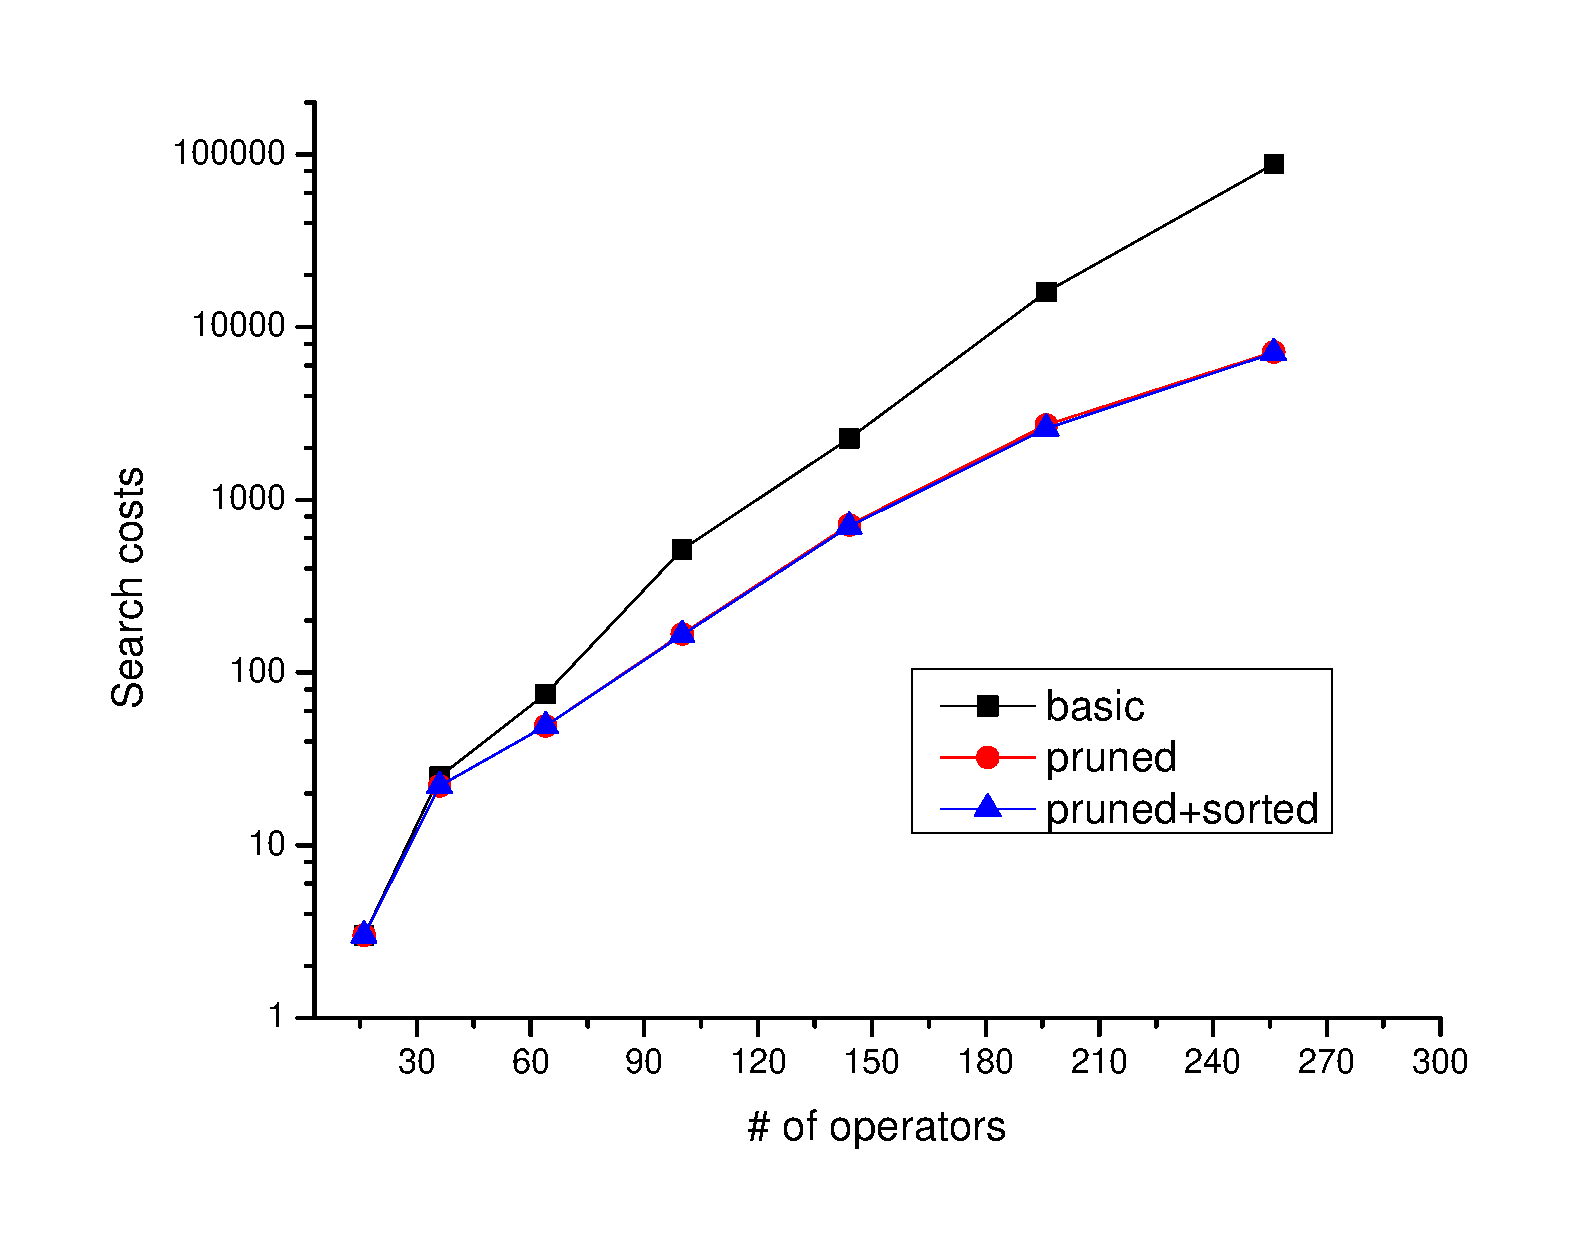
\includegraphics[width=0.324\textwidth]{figures2/eff_rand_num_sample0.5.eps}
\caption{Wrapped figure}
\label{fig:perf}
\end{wrapfigure}

\ifdefined\TTUT
\begin{figure}[!ht]
\begin{center}
    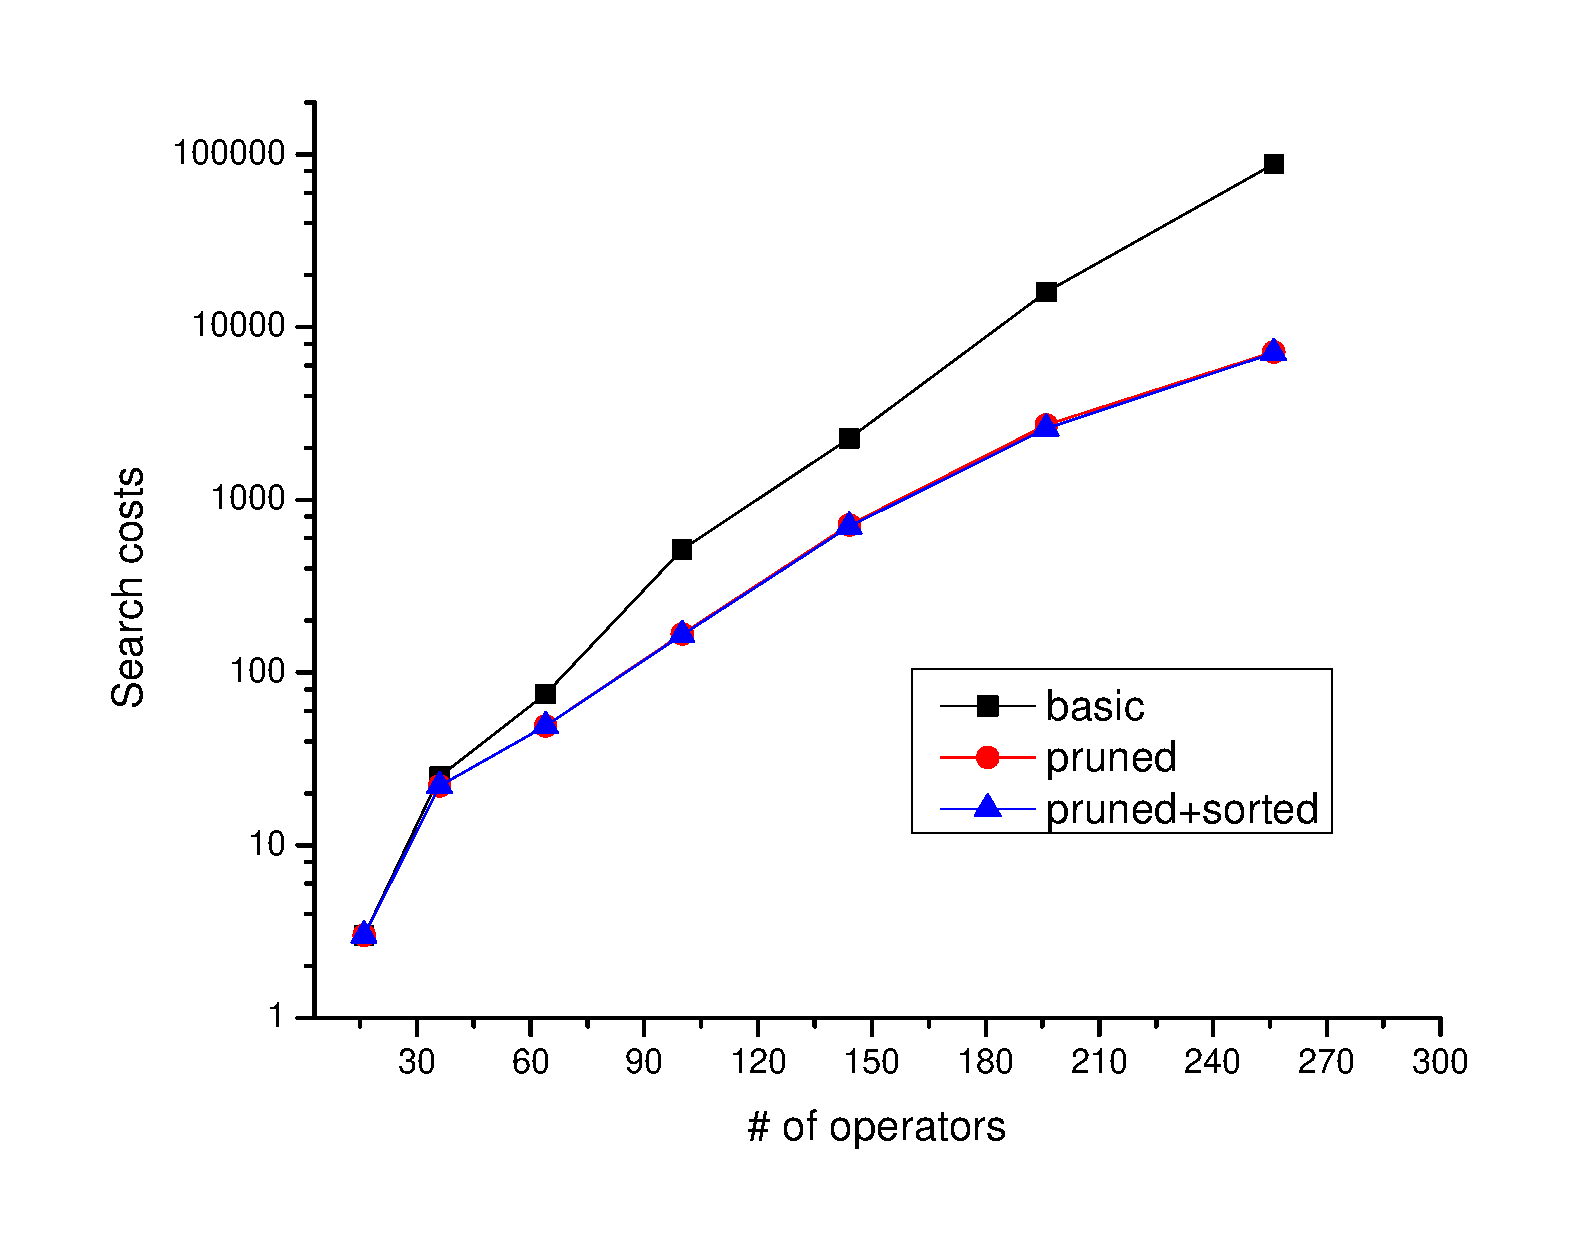
\includegraphics[angle=90, width=0.45\textwidth]{figures2/eff_rand_num_sample0.5.eps}%
\end{center}
%\vspace{-0.15in}
\caption{Easy figure}\label{fig:easy}
\vspace{-0.10in}\end{figure}

\begin{figure*}[!ht]
  \begin{center}
  %\goodgap
    \subfloat[Rotated]{%
      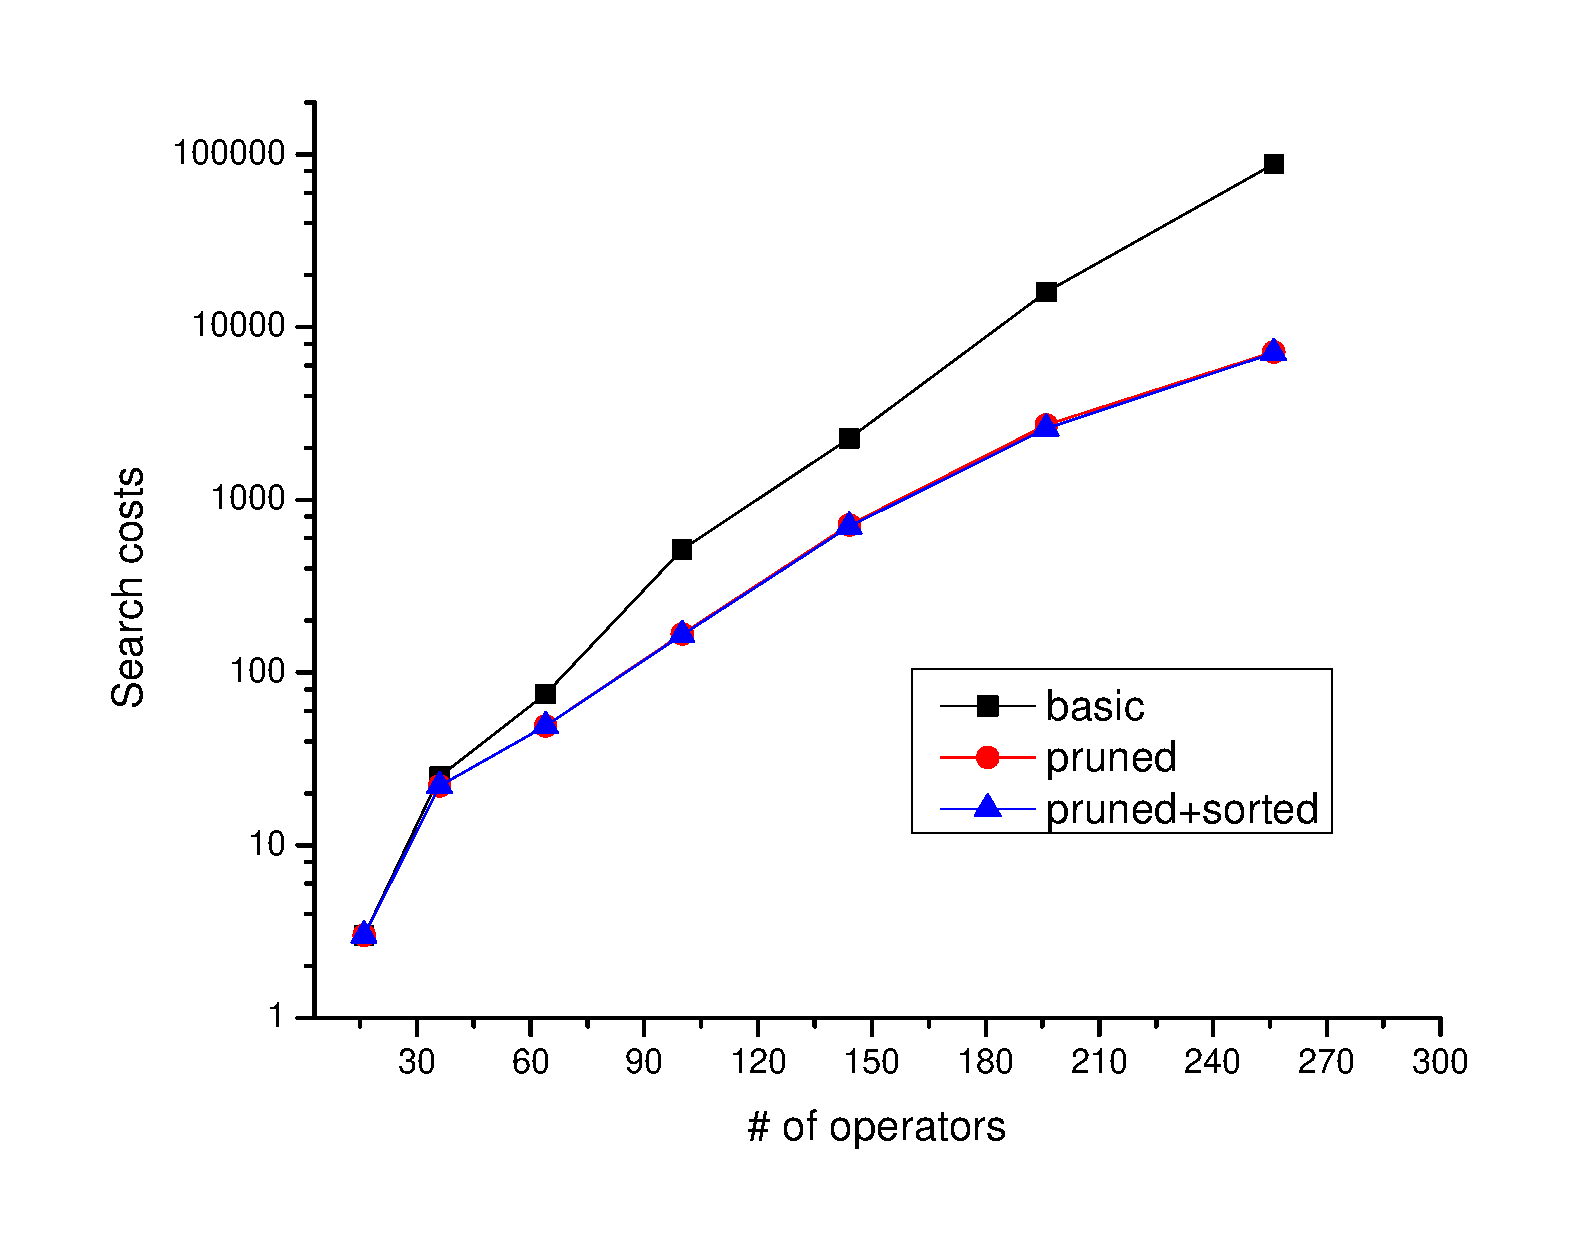
\includegraphics[angle=90, width=0.3\textwidth]{figures2/eff_rand_num_sample0.5.eps}%
      \label{exp:rand_num_1}%
    }%
    %\hspace{-0.2cm}%
    \subfloat[With more shared threads]{%
      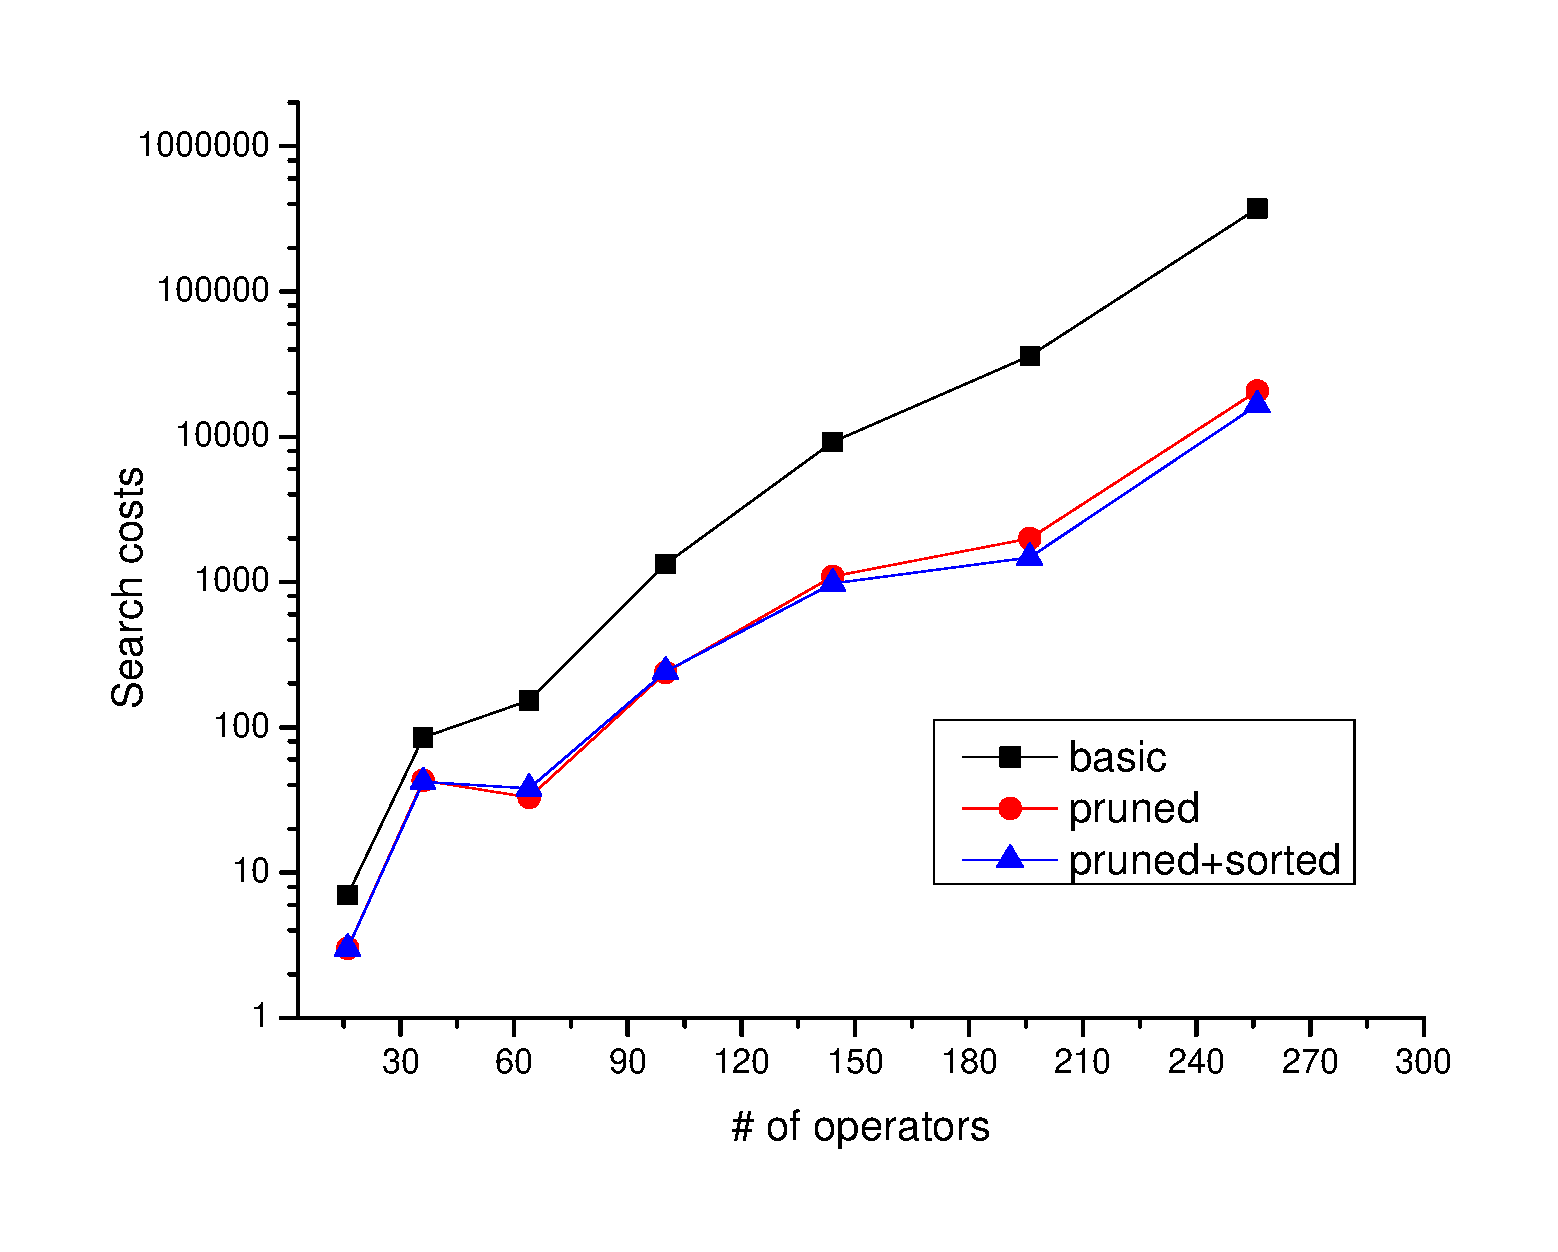
\includegraphics[width=0.3\textwidth]{figures2/eff_rand_num_sample2.eps}%
      \label{exp:rand_num_2}%
    }%
    \subfloat[With sample ratio]{%
      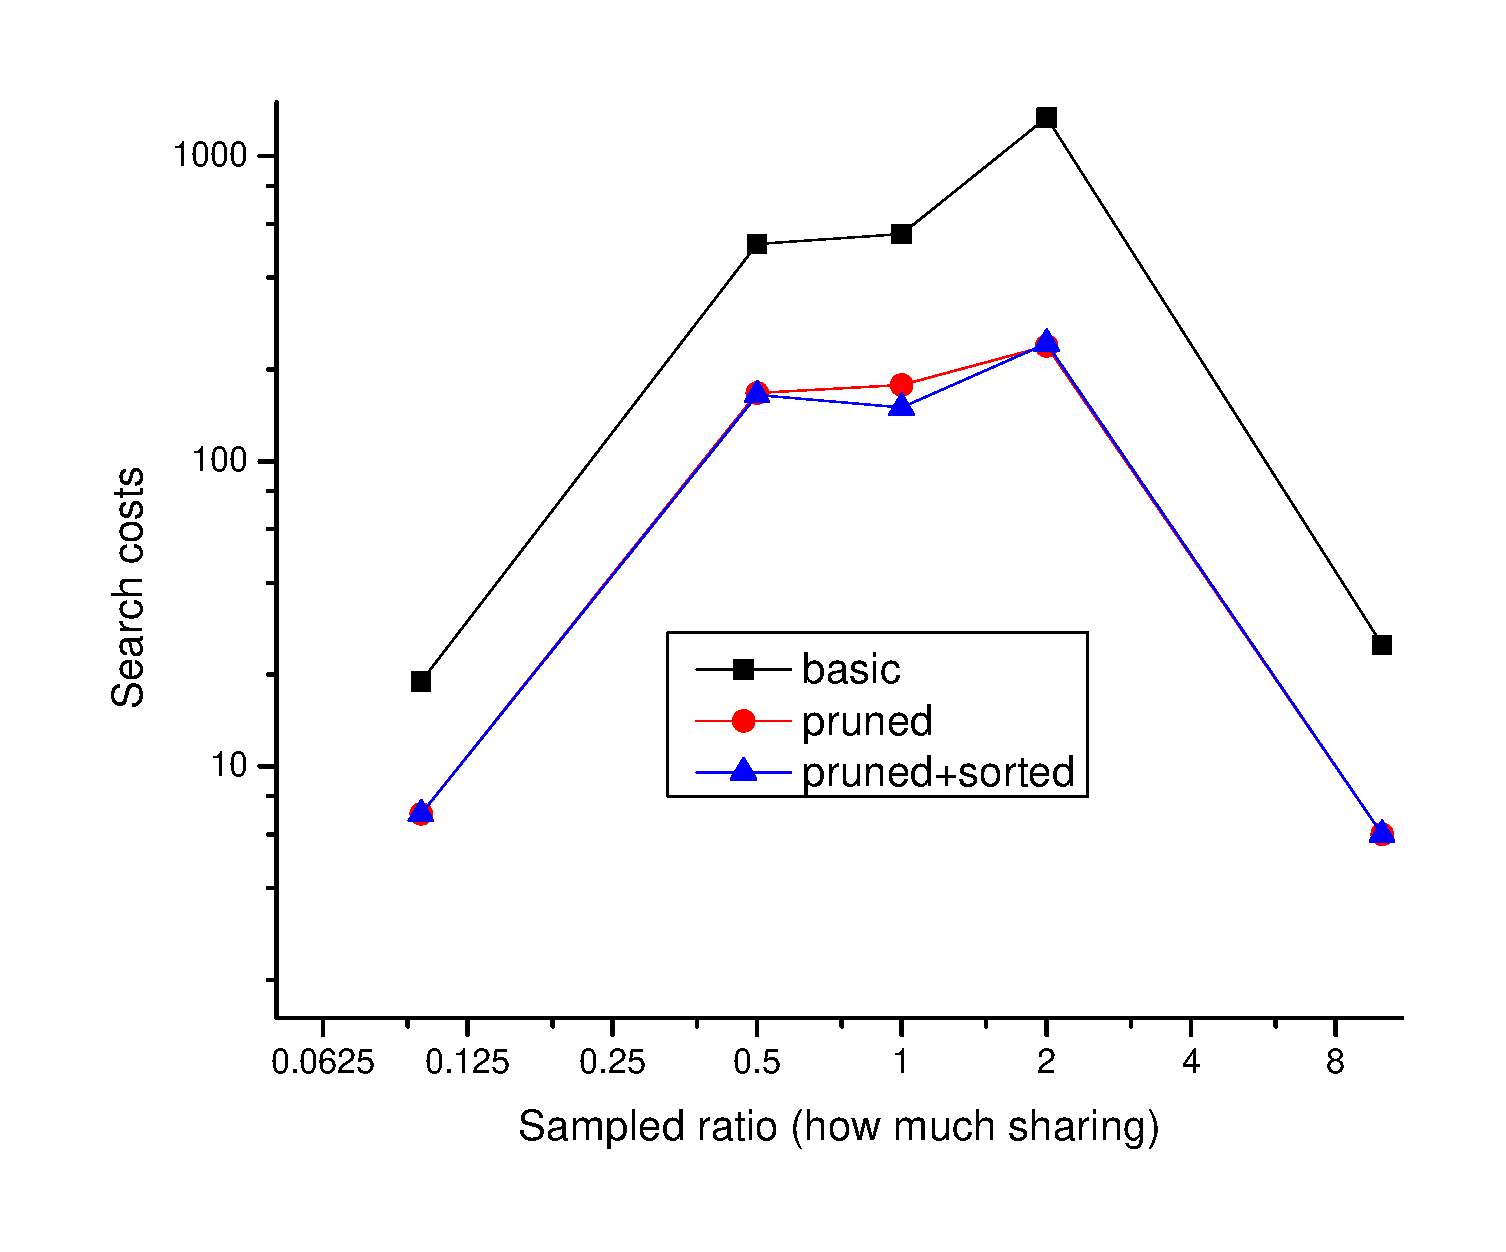
\includegraphics[width=0.3\textwidth]{figures2/eff_rand_sample_num10.eps}%
      \label{exp:rand_sample}%
    }%
  \end{center}%\vspace{-0.15in}
  \caption{Performance of optimization algorithm with random graph}\label{fig:complex}\vspace{-0.10in}
\end{figure*}
\fi

\subsection{algorithms}
\begin{algorithm}[h]
\caption{range-query(range $R$)}\small \label{alg:rangequery}
\begin{algorithmic}[1]
  \boldnext\State $\omega_R\leftarrow $ lowest-common-ancestor($R$) \Comment{comments: line number boldened}
  \State $\lambda\leftarrow $ DHT-lookup($f_{md}(\omega_R)$)
  \ForAll{$p \in P$} \Comment{comments: loop over all items}
    \State manipulate each term $p$
  \EndFor
  \If{$\lambda == NULL \And 1 \leq 0$}
      \State \Return lookup($R$.top\_left\_corner)
  \ElsIf{$R\subseteq{\lambda}$}
      \State \Return the keys of $\lambda$ that are in the range $R$
  \Else
      \State \Return recursive-forward($R$, $\omega_R$)
  \EndIf
\end{algorithmic}
\end{algorithm}

\subsection{equations}
\begin{eqnarray}
u &=& \sum_{l=0}^{n-1}{u_l} \mod{q} %\nonumber \\
=(\sum_{l=0}^{n-1}{ \sum_{j=0}^{c-1}{u_{l-j, j}} \mod{q}})\mod{q} \nonumber \\
&=& (\sum_{j=0}^{c-1}{ \sum_{l=0}^{n-1}{ u_{l-j, j} } })\mod{q} %\nonumber \\
=(\sum_{j=0}^{c-1}{ \sum_{i=-j}^{n-1-j}{ u_{i, j} } })\mod{q} \nonumber \\
&=& (\sum_{j=0}^{c-1}{\sum_{i=0}^{n-1}{ u_{i, j} } }) mod q
= (\sum_{i=0}^{n-1}{ \sum_{j=0}^{c-1}{ u_{i, j} }\mod{q} })\mod{q} \nonumber \\
&=& \sum_{i=0}^{n-1}{ v_i }\mod{q} = \sum_{i=0}^{n-1}{ v_i } = v
\end{eqnarray}

With right brace
\begin{eqnarray}
\underline{\sigma}, \epsilon \rightarrow{}\underline{\beta_*}
\begin{cases}
\begin{rcases}
\begin{rcases}
& \sum_{\forall\beta_*>1}{(\beta_* - 1)} \\
& \sum_{\forall\beta_*<1}{(1 - \beta_*)} \\  
\end{rcases} \rightarrow{} \underline{X_1}\% \\
\sum_{\beta_*<1}{1} \rightarrow{} \underline{X_2}\%
\end{rcases}
\end{cases}
 \rightarrow{\beta}
\end{eqnarray}

\subsection{listing}
\lstset{language=SQL, style=Oracle, caption={Rewritten query against a single view table},label=sql:rewritten}
\lstset{frame=lrbt,xleftmargin=\fboxsep,xrightmargin=-\fboxsep} %with bounding box at l(eft)r(right)b(ottom)t(op)
%or you can replace it with "frame=single"
\begin{lstlisting}
  SELECT A, C FROM viewtable
  ORDER BY C LIMIT arg.k
\end{lstlisting}

\definecolor{mygreen}{rgb}{0,0.6,0}
\begin{figure}[h!]
%\begin{scriptsize}
%\begin{tabular}{cc}
%\begin{minipage}{.5\textwidth}
\lstset{ %
  backgroundcolor=\color{white},   % choose the background color; you must add \usepackage{color} or \usepackage{xcolor}
  %basicstyle=\footnotesize\ttfamily,        % the size of the fonts that are used for the code
  basicstyle=\scriptsize\ttfamily,        % the size of the fonts that are used for the code
  breakatwhitespace=false,         % sets if automatic breaks should only happen at whitespace
  breaklines=true,                 % sets automatic line breaking
  captionpos=b,                    % sets the caption-position to bottom
  commentstyle=\color{mygreen},    % comment style
  deletekeywords={...},            % if you want to delete keywords from the given language
  escapeinside={(*}{*)},          % if you want to add LaTeX within your code
  extendedchars=true,              % lets you use non-ASCII characters; for 8-bits encodings only, does not work with UTF-8
  %frame=single,                    % adds a frame around the code
  keepspaces=true,                 % keeps spaces in text, useful for keeping indentation of code (possibly needs columns=flexible)
  keywordstyle=\color{blue},       % keyword style
  language=Java,                 % the language of the code
  morekeywords={*,...},            % if you want to add more keywords to the set
  numbers=left,                    % where to put the line-numbers; possible values are (none, left, right)
  numbersep=5pt,                   % how far the line-numbers are from the code
  numberstyle=\scriptsize\color{black}, % the style that is used for the line-numbers
  rulecolor=\color{black},         % if not set, the frame-color may be changed on line-breaks within not-black text (e.g. comments (green here))
  showspaces=false,                % show spaces everywhere adding particular underscores; it overrides 'showstringspaces'
  showstringspaces=false,          % underline spaces within strings only
  showtabs=false,                  % show tabs within strings adding particular underscores
  stepnumber=1,                    % the step between two line-numbers. If it's 1, each line will be numbered
  stringstyle=\color{mymauve},     % string literal style
  tabsize=2,                       % sets default tabsize to 2 spaces
  title=\lstname,                  % show the filename of files included with \lstinputlisting; also try caption instead of title
  moredelim=[is][\bf]{*}{*},
}
\begin{lstlisting}
public void OnTouchEvent(MotionEvent e) {
Bitmap LoadPicture(String path) {
    ...
    *Bitmap bm = BitmapFactory.decodeFile(file)*;
    return bm;
}

void EditPicture(Bitmap bm) {
    //heavy computational picture editing
    int i = 10 (* $*$ *); //escape to plot * literatelly instead of bolden text
    bm.getPixels(pix, 0, mPhotoWidth, 0, 0, mPhotoWidth, mPhotoHeight);
    for(every pixel) {
      ...
    }  
    
    //embed location information into picture
    (* $*$*)Location loc = getLastKnownLocation(Provider)*;
    (* $*$*)double longitude = loc.getLongitude()*;
    (* $*$*)double latitude = loc.getLatitude()*;
    (* $*$*)EmbedLocation(bm, longitude, latitude);*
}
\end{lstlisting}
%\end{minipage}
%\end{tabular}
%\end{scriptsize}
\caption{Privacy-preserving Offloading Example}
\label{figure:MotivatingExample}
\end{figure}


\subsection{fbox}
\begin{center}
\fbox{This is a sample statement}
\end{center}

\begin{center}
\fbox{\parbox{0.90\linewidth}{
This is a long long long statement: 
Blah blah blah blah 
Blah blah blah blah 
Blah blah blah blah 
Blah blah blah blah 
Blah blah blah blah 
Blah blah blah blah 
Blah blah blah blah 
Blah blah blah blah 
}}
\end{center}



\subsection{misc}
\begin{itemize}
  \item caret $\textrm{\^{}}$ 
  \item cmark $\cmark$ and xmark $\xmark$
  \item bold math type $\boldsymbol{<v_0, k>}$
  \item use other than default font size: {``\fontsize{8.5}{9} this's in font size 8.5''}. (second param. should be 1.2$\times$ first param. which is font size
  \item show tilde in url, use \textasciitilde{} rather than \~{}
  \item strike out text, \sout{text/$12$ removed}
  \item color, {\color{red}red}{\color{green}green}
  \item[$\bullet$] big bullet on each item
  \item circled text \circled{2}
  \item A white number inside a black circle: \ballnumber{37}
  \item empty set (beautiful version) $\varnothing$ (needs ``\\usepackage\{amssymb\}''), which renames emptyset, $\emptyset$
  \item stackrel $\stackrel[c]{a}{=}$
\end{itemize}

citation for long breakable url~\cite{me:mssgx}


  \input{text/experiment.tex}
  \input{text/casestudy.tex}
  \input{text/relatedwork.tex} %related work should always be the last to write.
  \input{text/conclusion.tex}
\fi

\ifdefined\TTSTYLETARGETonecolumn
  \bibliographystyle{IEEEtran}
\fi
\ifdefined\TTSTYLETARGETieeetran
  \bibliographystyle{IEEEtran}
\fi
\ifdefined\TTSTYLETARGETsigalternate
  \bibliographystyle{abbrv}
\fi
\ifdefined\TTSTYLETARGETsig
  \bibliographystyle{abbrv}
\fi
\ifdefined\TTSTYLETARGETusenix
  \bibliographystyle{acm}
\fi

\ifdefined\TTSTYLETARGETreport
  \printbibliography
%note the list of bib is mentioned in sty/usepackage_config.tex
\else
  \bibliography{ads,lsm,bkc,odb,cacheattacks,sc,crypto,sgx,diffpriv,txtbk,distrkvs,vc,yuzhetang}
\fi

\ifdefined\TTSTYLETARGETsigalternate
  \appendix
\else
 \ifdefined\TTSTYLETARGETusenix
   \appendix
 \else
  \ifdefined\TTSTYLETARGETvldb
    \appendix
  \else
  \ifdefined\TTSTYLETARGETreport
    \appendix
  \else
    \ifdefined\TTSTYLETARGETllncs
      \appendix
    \else
      \appendices
    \fi
  \fi
 \fi
\fi
\fi

\input{text/appendix.tex}
\ifdefined\TTUT
\fi

\end{document}



